%************************************************
\chapter{Desarrollo}\label{ch:desarrollo}
%************************************************

En la primer sección de este capítulo se brindarán detalles del prototipo de dispositivo de medición mediante luz estructurada, junto con las características de sus principales componentes. 
En la segunda sección se justificará la elección de los patrones de luz estructurada que se utilizarán y se explicará de manera simple la forma en que se usan, siendo el punto más importante su decodificación de manera robusta. 
En la tercer sección se tratará la obtención de la nube de puntos en tres dimensiones a partir del uso de las imagenes de los patrones decodificados. 
La sección siguiente se dedicará específicamente al proceso de calibración y las herramientas dedicadas para tal fin. 
Finalmente en la última sección del capítulo se analizarán las más importantes limitaciones del dispositivo.

\section{Prototipo}
El prototipo desarrollado cuenta con dos cámaras y un proyector, como se muestra en la \autoref{fig:prototypeDiagram}.

\begin{figure}[!bth]
    \myfloatalign
        {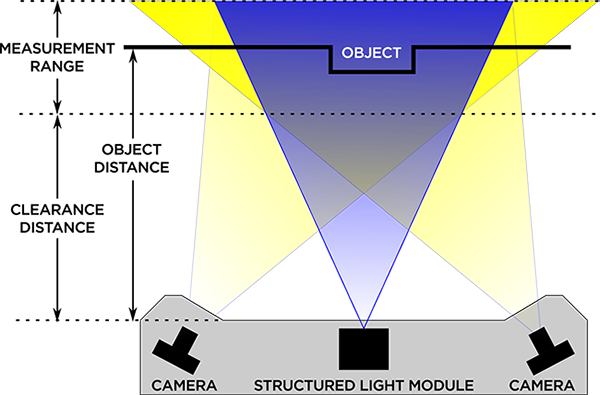
\includegraphics[width=1.0\linewidth]{images/lmi3d/Gocator-3100-howitworks}}
        \caption{Esquema del prototipo}
        \label{fig:prototypeDiagram}
\end{figure}

\subsection{Componentes}
Los principales componentes del prototipo desarrollado son:

\begin{itemize}
    \item cámara Point Grey Chameleon CMLN-13S2M-CS \footnote{\url{http://ww2.ptgrey.com/USB2/chameleon}}
    \item cámara Lumenera LM165M \footnote{\url{http://www.lumenera.com/products/industrial-cameras/lm165.php}}
    \item proyector Texas Instruments DLP Pico Projector Development Kit \footnote{\url{http://www.ti.com/tool/dlp1picokit}}
\end{itemize}

Se elige la utilización de cámaras en escala de grises (no color) ya que estas son más eficientes respecto a la adquisición de la luz y tienen menor ruido. Esto se debe en gran medida a que las cámaras monocromáticas no incorporan lo que se conoce como filtro de bayer, el cual es necesario para obtener imágenes color (existen otros métodos para obtener imágenes color, pero éste es el más utilizado). Las cámaras brindan la posibilidad de ser controladas por una señal de trigger hardware, sin embargo para las pruebas no se utiliza de esta manera, sino que son controladas y sincronizadas completamente por software.

El proyector es de bajo consumo y reducidas dimensiones, pero también de baja resolución: solamente 320 x 480 pixels. La ventaja de este proyector está en la utilización de tecnología DLP de Texas Instruments. Básicamente se trata de un proyector que genera la imagen a partir de una fuente de luz LED y una grilla de espejos en miniatura. El diagrama del funcionamiento de un espejo puede verse en la \autoref{fig:dlpMirrorOpticalDiagram}. Este tipo de tecnología posibilita generar patrones binarios con frecuencias mayores a 2 KHz. Si bien en el prototipo no estamos utilizando esta ventaja (ya que se lo utiliza como un proyector común de computadora), se tiene en cuenta que el dispositivo brinda esta posibilidad, la cual puede ser aprovechada mediante el uso de cámaras de alta velocidad y sincronizadas por hardware.

\begin{figure}[!bth]
    \myfloatalign
        {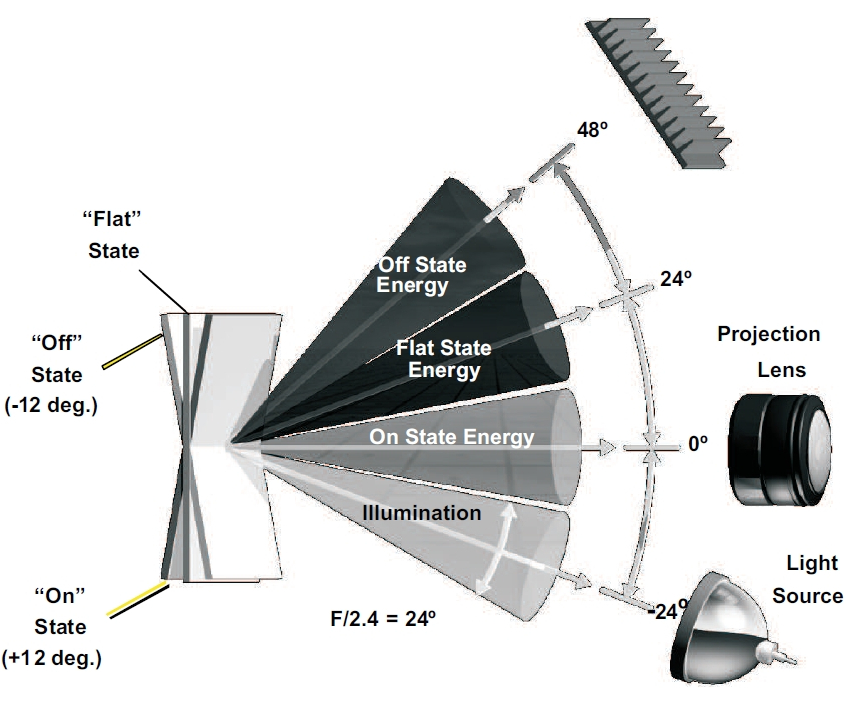
\includegraphics[width=1.0\linewidth]{images/DLP_mirrorOpticalDiagram}}
        \caption{Diagrama de funcionamiento de la tecnología DLP}
        \label{fig:dlpMirrorOpticalDiagram}
\end{figure}

\section{Proyección y decodificación de los patrones}
Para la codificación y decodificación se parte de la suposición de que el objeto se mantiene estático durante todo el período de escaneado.

La codificación que utilizaremos se basa en patrones binarios donde cada patrón representa un bit del código binario. La obtención de un código único (de más de un bit) se realiza mediante multiplexación en tiempo: se toma una imagen de cada patrón proyectado de manera sucesiva. Se utiliza código binario gray por sus ventajas ya nombradas en la \autoref{sec:structuredLightBinary1DPatterns}. 

La elección de utilizar patrones binarios se debe principalmente a que este tipo de patrones brinda una codificación única para cada pixel, lo que hace que su decodificación sea muy robusta, y por otro lado también es relativamente simple de implementar. El uso de un patrón del tipo \emph{phase shift} puede brindarnos una mejor resolución lateral, y se podría aprovechar la ventaja que nos brinda el conocer que los objetos que se desean medir tienen superficies suaves y geometrías simples. Sin embargo el hecho de que no podemos permitirnos ambiguedades en la decodificación nos obligaría a incluir al menos un patrón de algún otro tipo que permita establecer un punto de referencia, ya que se debe conocer la fase absoluta en al menos un punto a partir del cual continuar la decodificación de la fase absoluta para todos los pixels. Por otro lado la resolución espacial que se logra resulta suficiente, ya que no es un factor crítico la detección de características puntuales. 

En principio, para facilitar la detección de las zonas donde el patrón está presente y es visible por la cámara y para determinar un umbral mínimo de la \emph{calidad} del pixel, se utiliza un patrón extra que es completamente blanco, y su inverso completamente negro. Este patrón se utiliza como \emph{máscara} para procesar solamente los pixels que contienen información útil.

Por otro lado, para poder discernir claramente cual es el valor binario para cada pixel, se utiliza el patrón junto a su patrón inverso. De esta forma el valor binario $1$ corresponde a un valor alto en la imagen patrón y un valor bajo en la imagen del patrón inverso. De manera similar, el valor binario $0$ corresponde entonces a un valor bajo en la imagen del patrón y un valor alto en la imagen de su inverso. 





\begin{figure}[!bth]
    \myfloatalign
        \subfloat{
            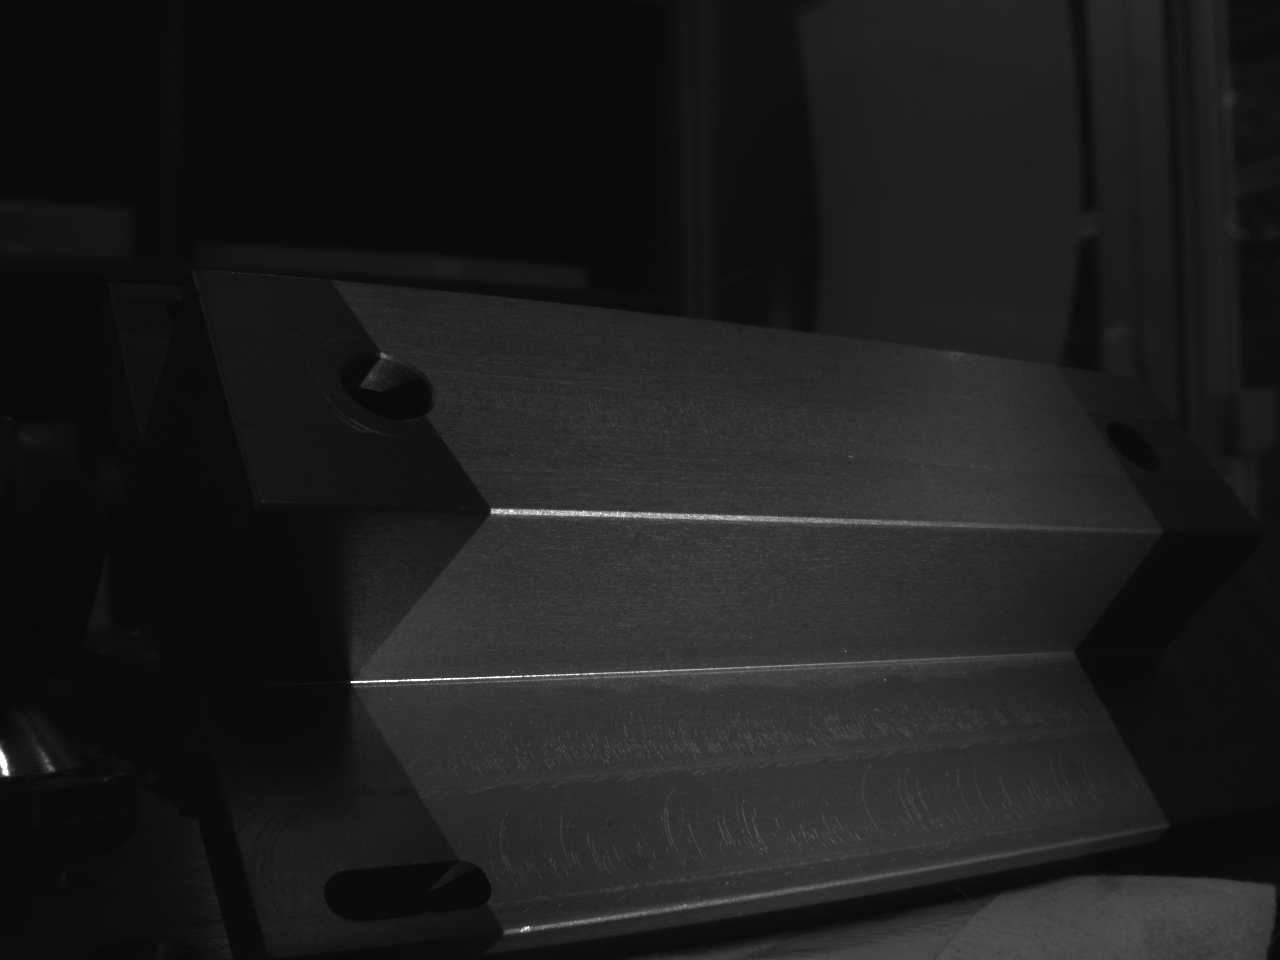
\includegraphics[width=0.49\linewidth]{images/snapshots_scan/SIMULATED-LEFT-LUMENERA-SN8010129/gray_00}
            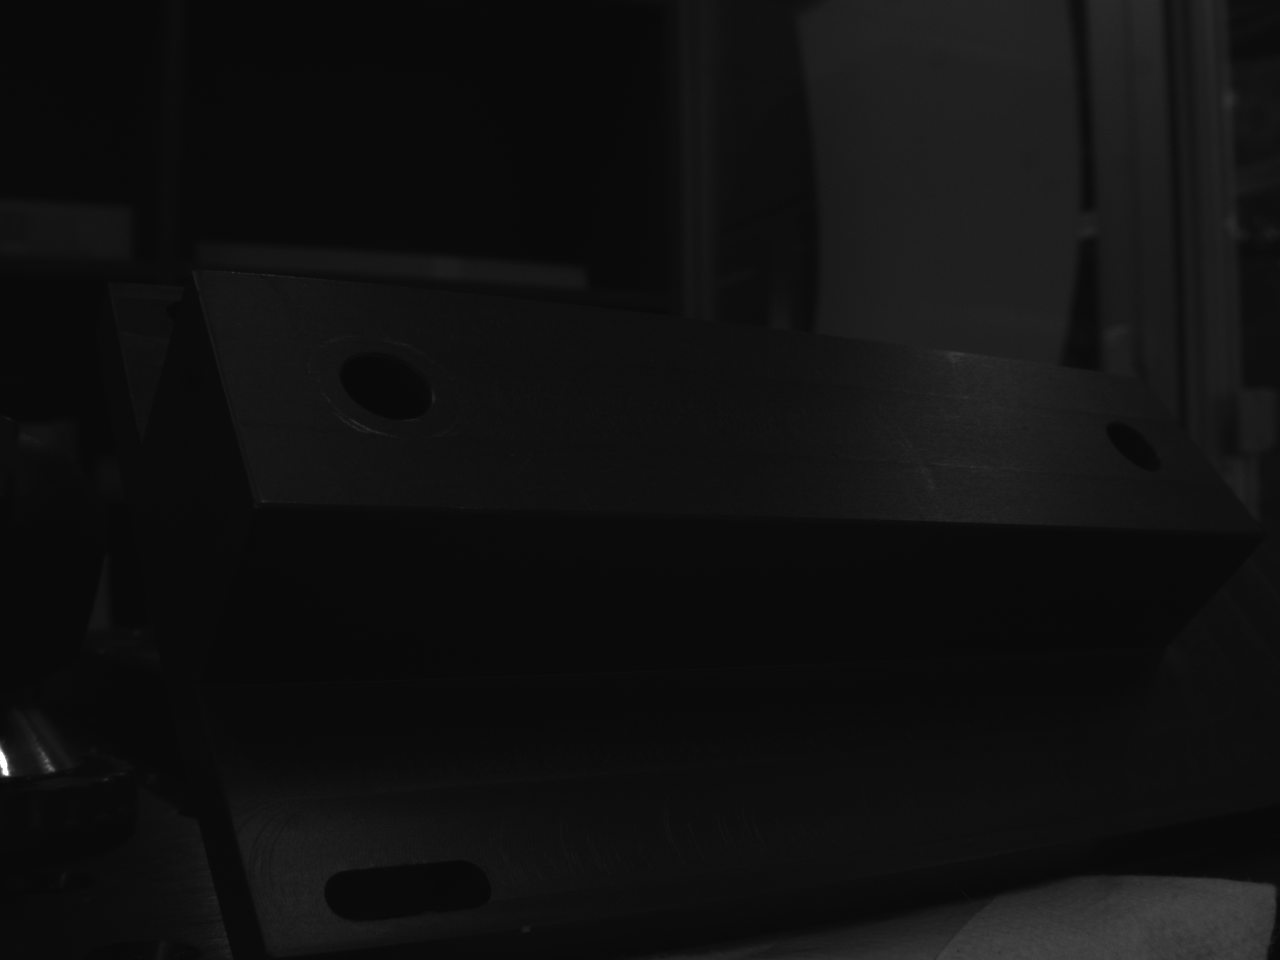
\includegraphics[width=0.49\linewidth]{images/snapshots_scan/SIMULATED-LEFT-LUMENERA-SN8010129/gray_00_inv}
        }
        \\
        \subfloat{
            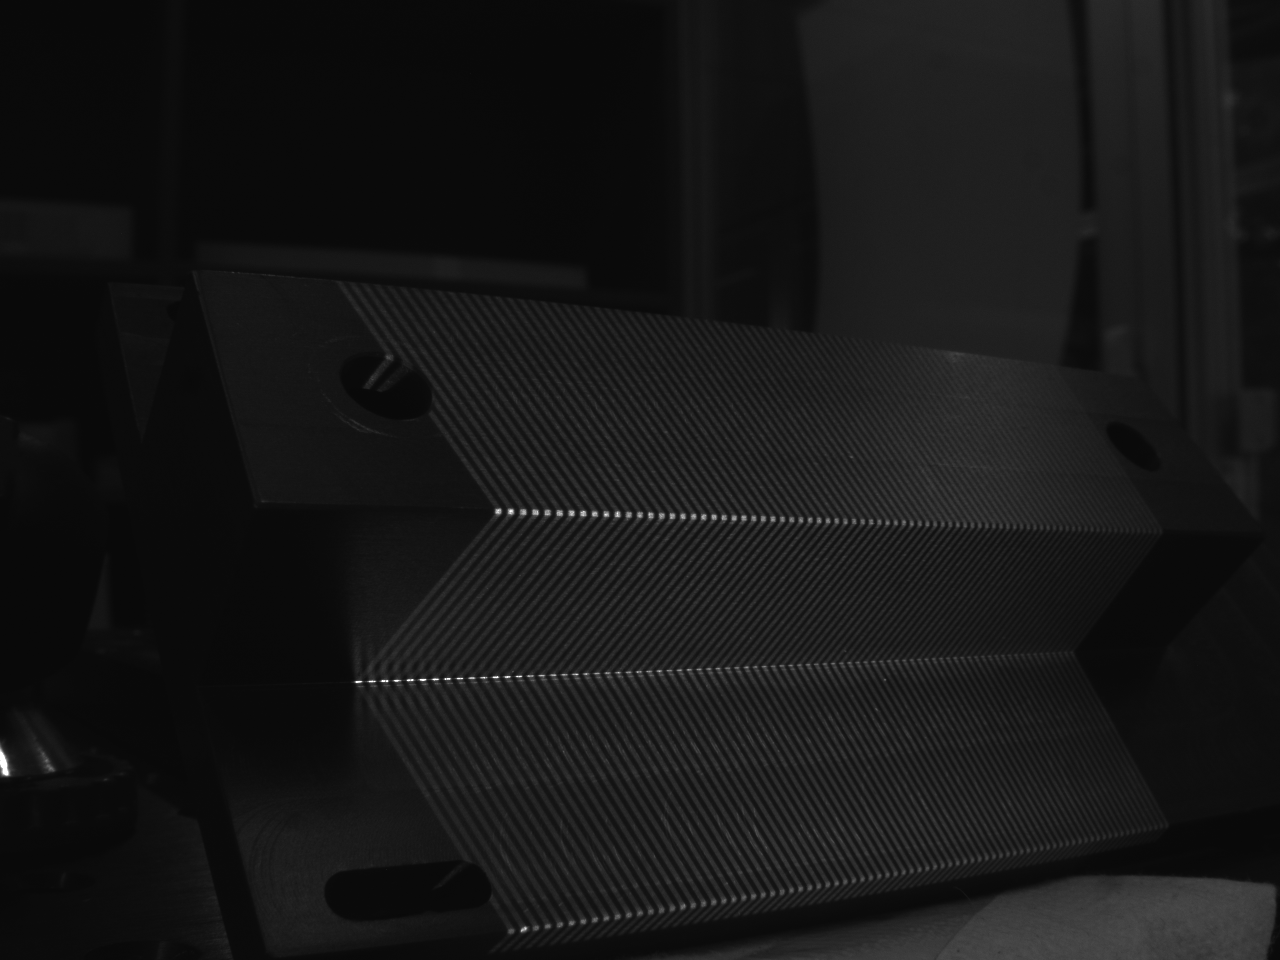
\includegraphics[width=0.49\linewidth]{images/snapshots_scan/SIMULATED-LEFT-LUMENERA-SN8010129/gray_01}
            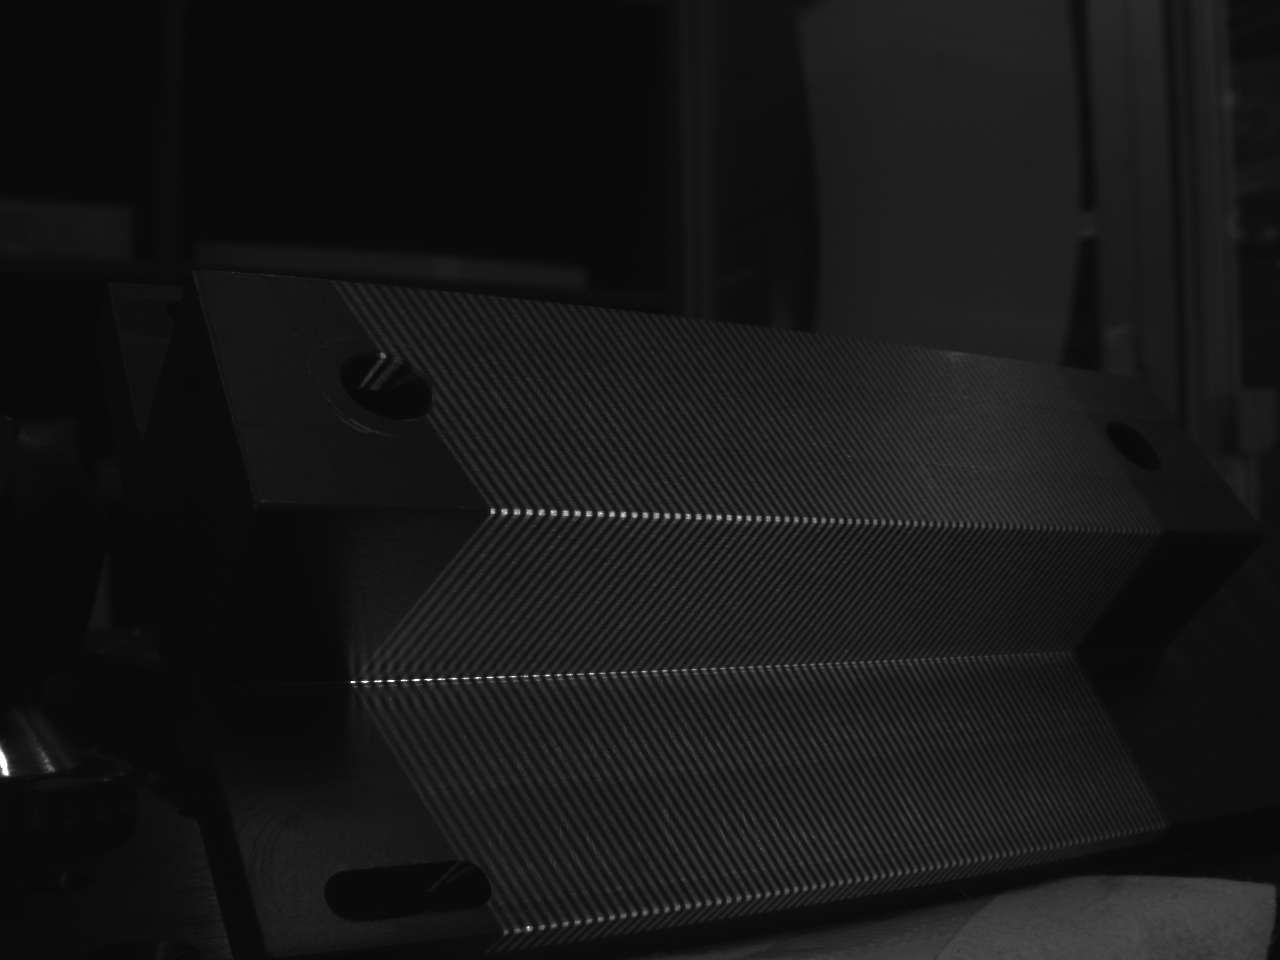
\includegraphics[width=0.49\linewidth]{images/snapshots_scan/SIMULATED-LEFT-LUMENERA-SN8010129/gray_01_inv}
        }
        \\
        \subfloat{
            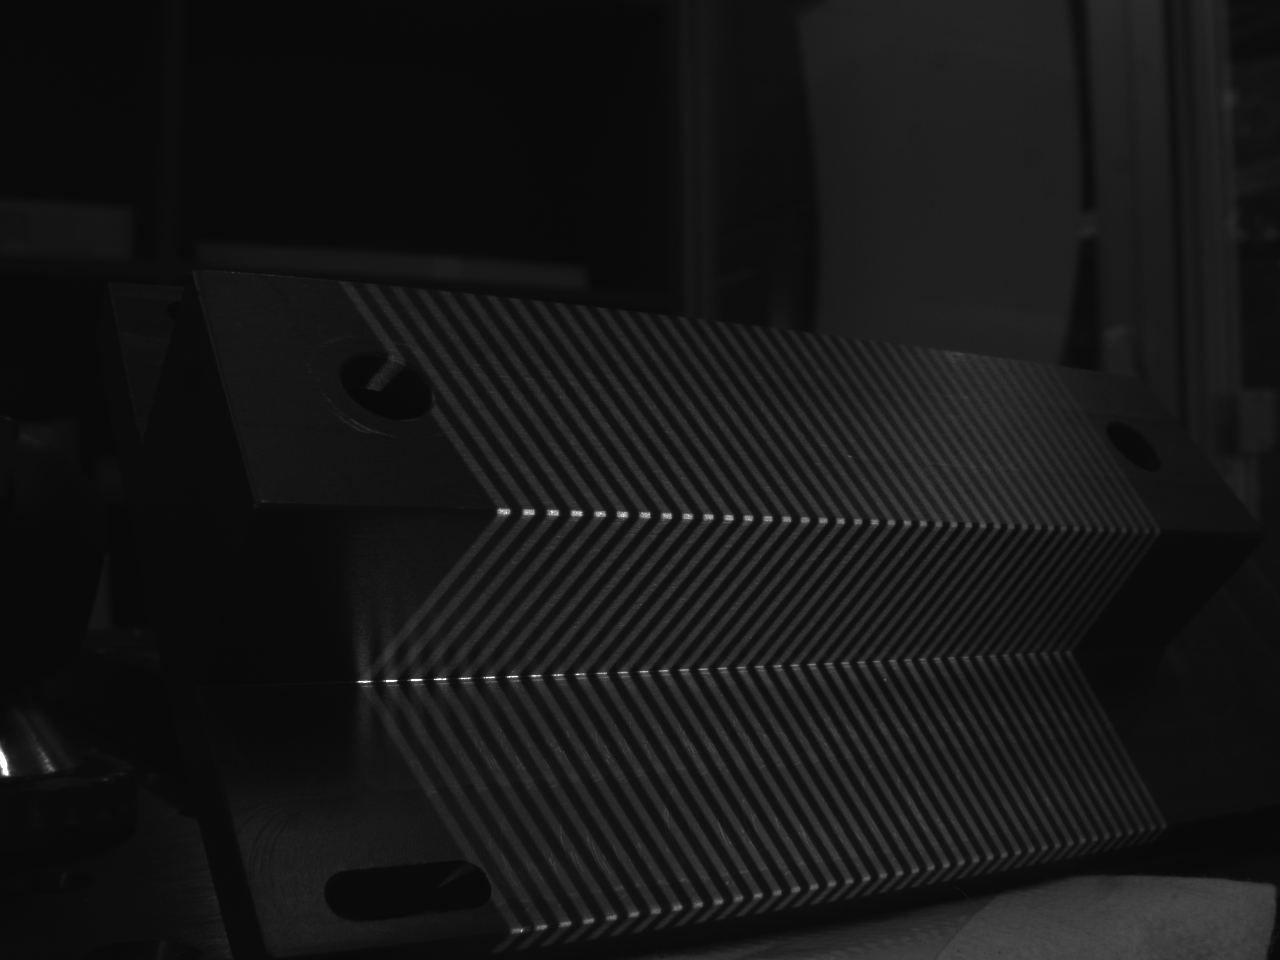
\includegraphics[width=0.49\linewidth]{images/snapshots_scan/SIMULATED-LEFT-LUMENERA-SN8010129/gray_02}
            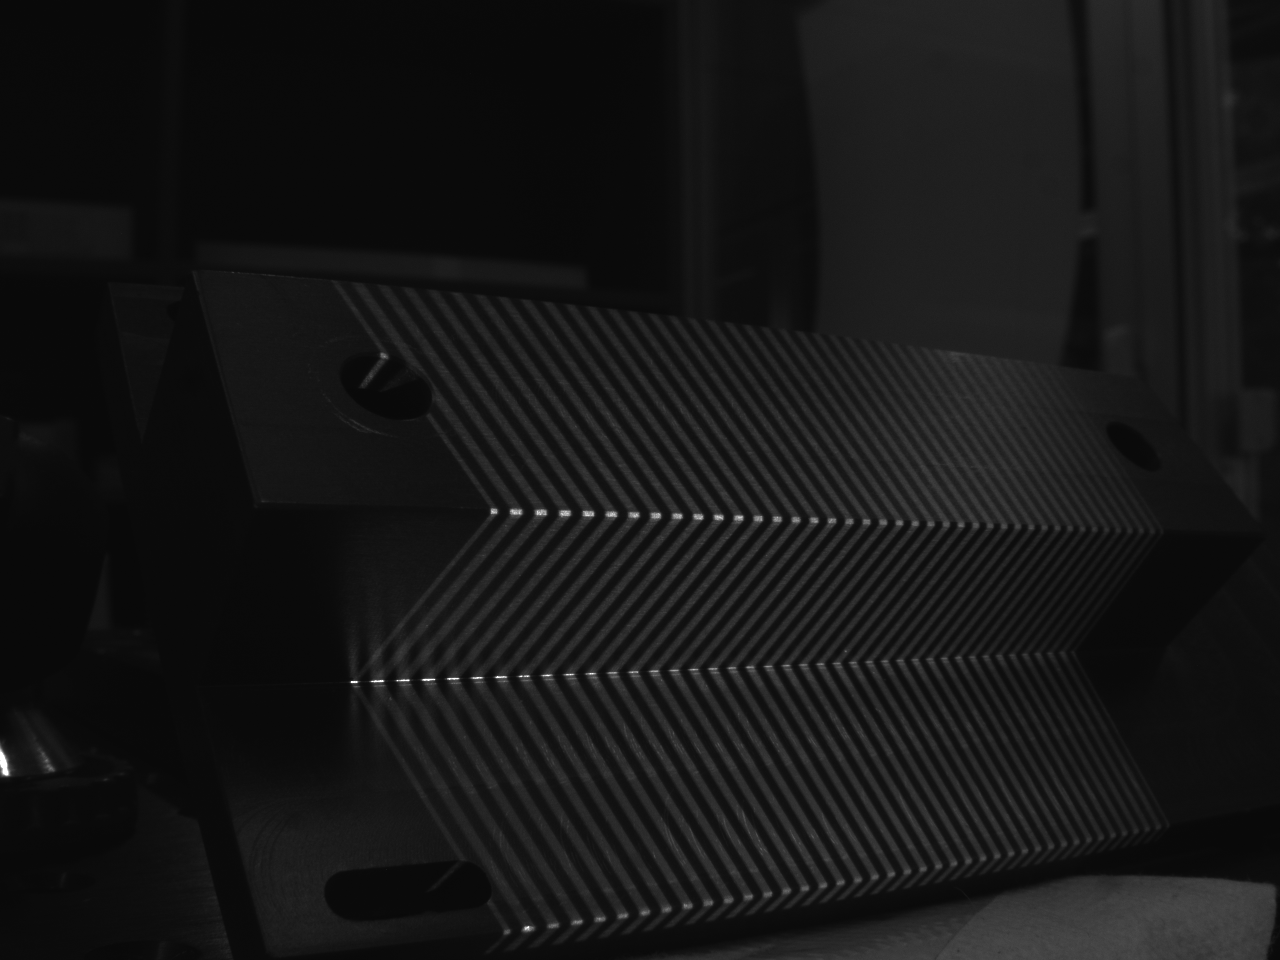
\includegraphics[width=0.49\linewidth]{images/snapshots_scan/SIMULATED-LEFT-LUMENERA-SN8010129/gray_02_inv}
        }
        \\
        \subfloat{
            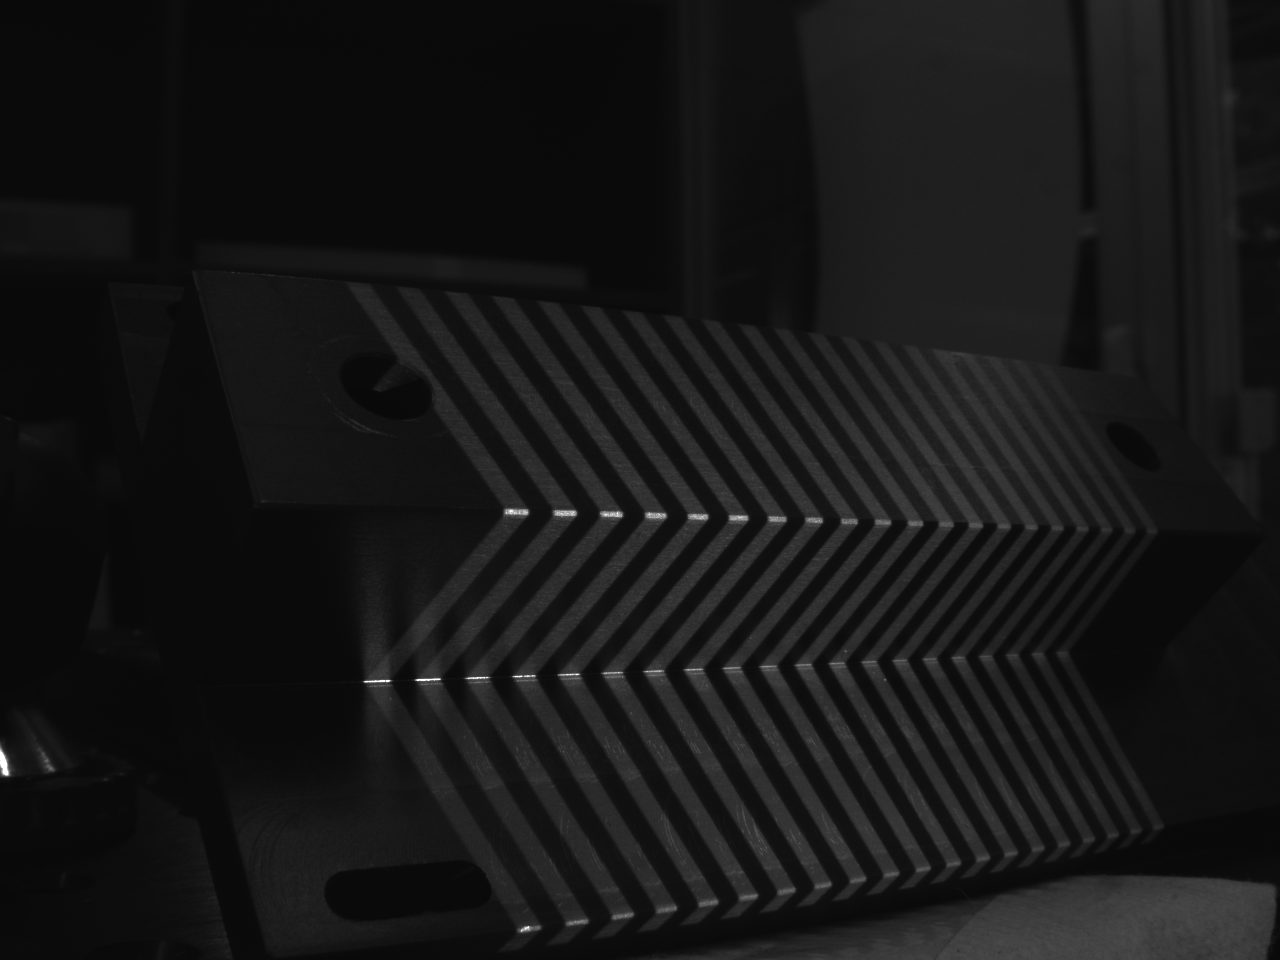
\includegraphics[width=0.49\linewidth]{images/snapshots_scan/SIMULATED-LEFT-LUMENERA-SN8010129/gray_03}
            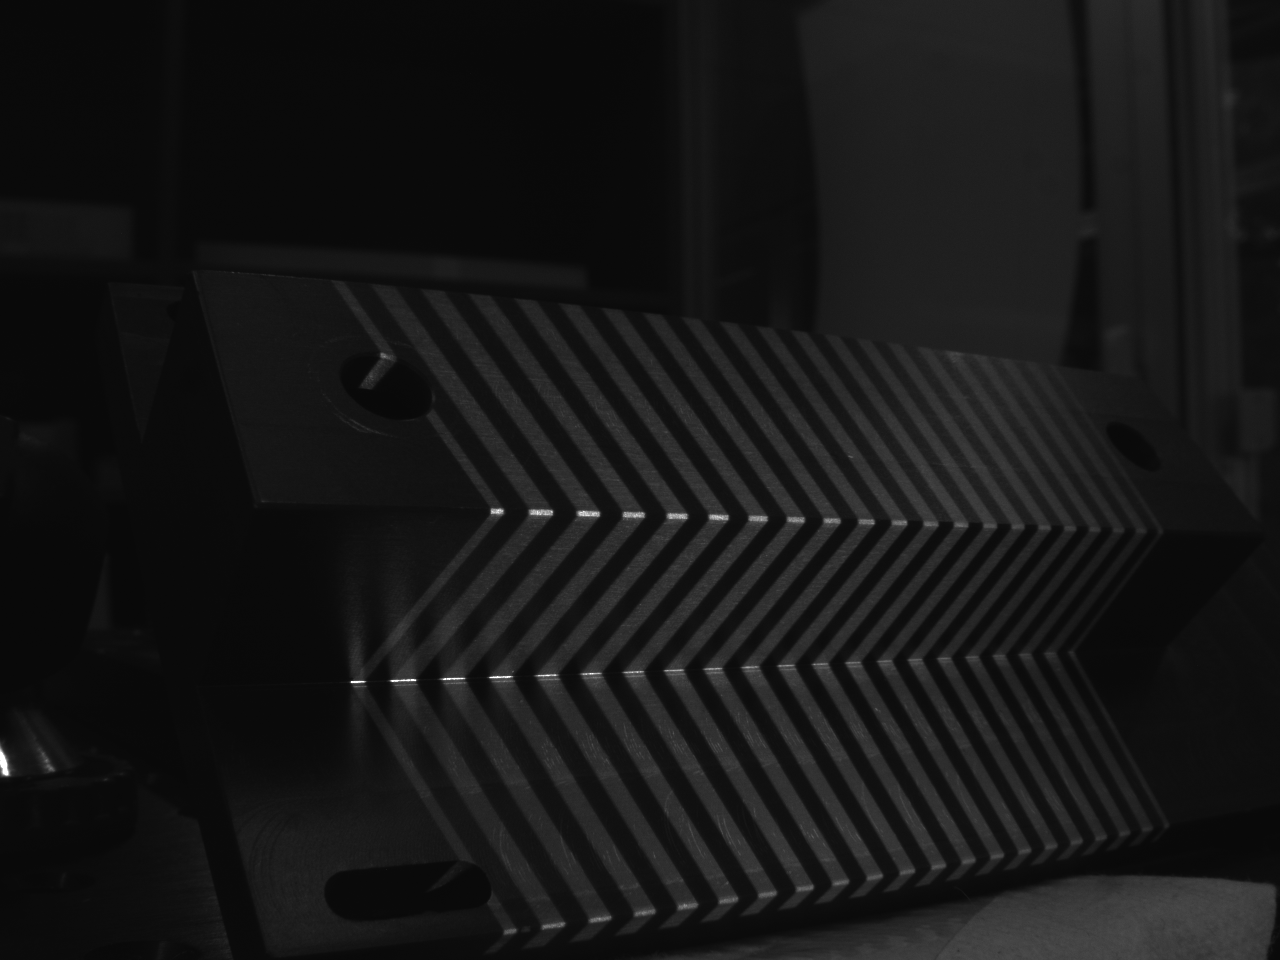
\includegraphics[width=0.49\linewidth]{images/snapshots_scan/SIMULATED-LEFT-LUMENERA-SN8010129/gray_03_inv}
        }
        \\
        \subfloat{
            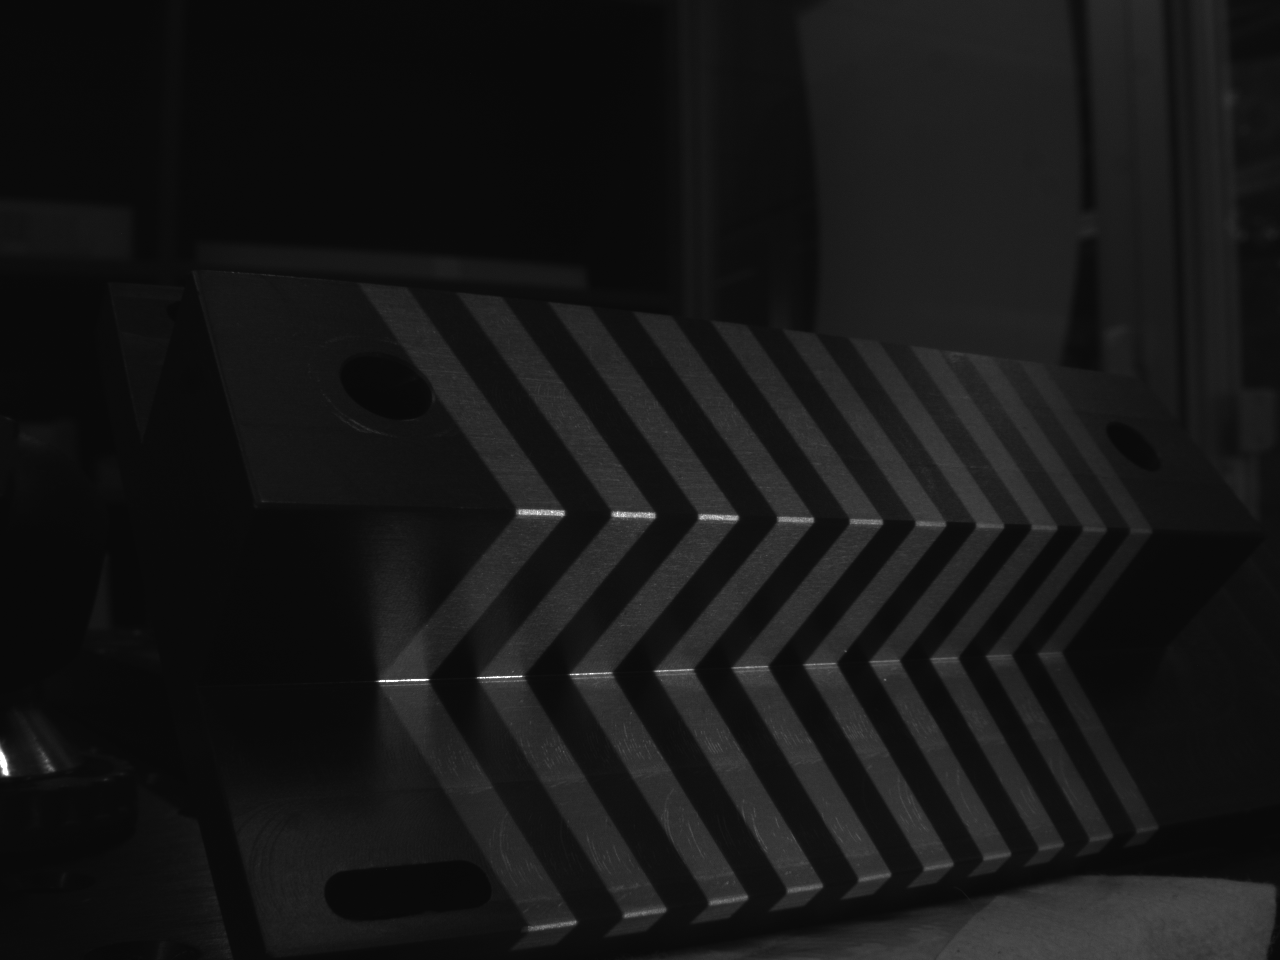
\includegraphics[width=0.49\linewidth]{images/snapshots_scan/SIMULATED-LEFT-LUMENERA-SN8010129/gray_04}
            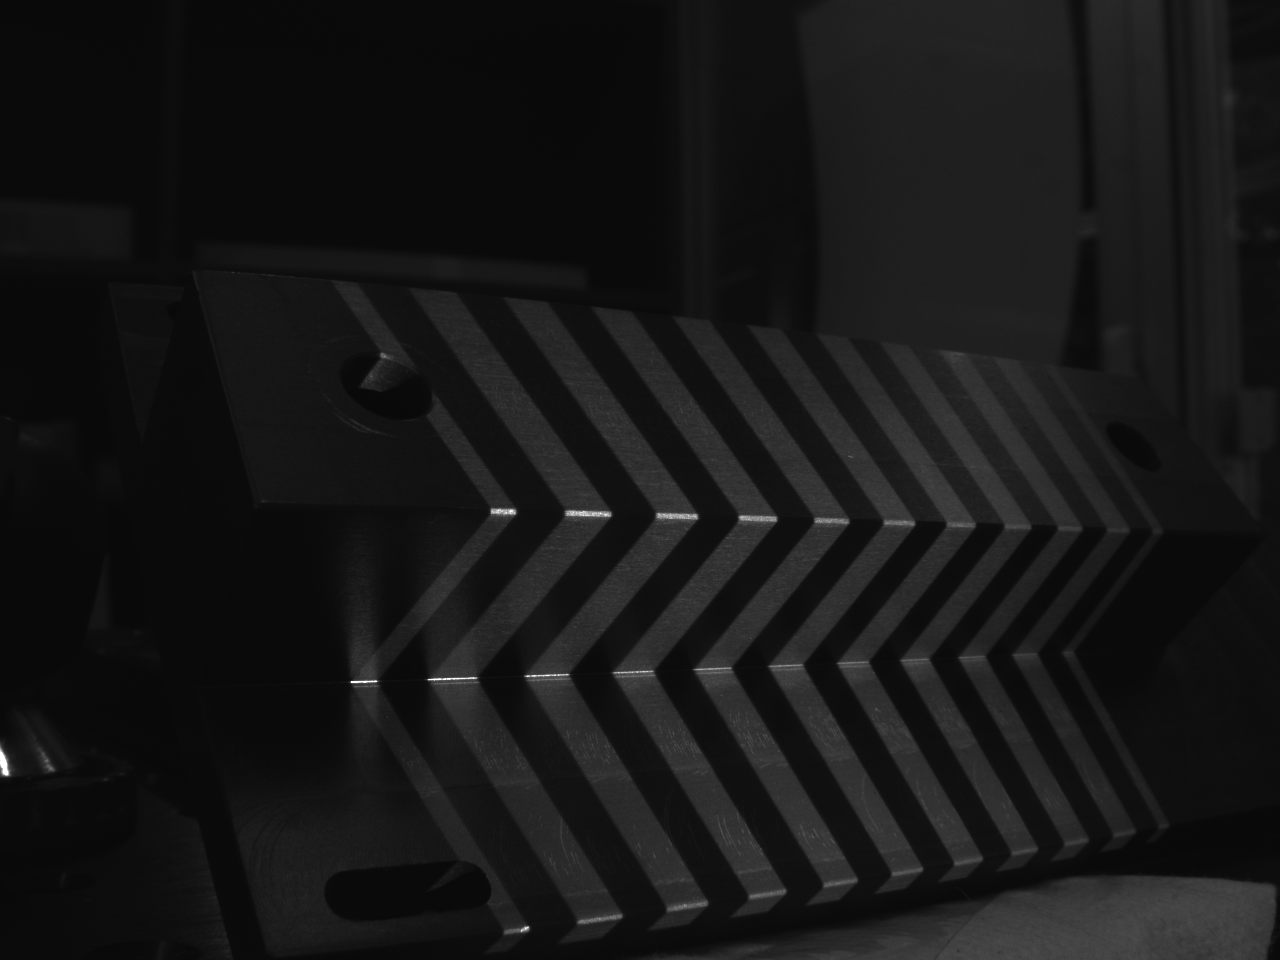
\includegraphics[width=0.49\linewidth]{images/snapshots_scan/SIMULATED-LEFT-LUMENERA-SN8010129/gray_04_inv}
        }
        \caption{Cámara izquierda: 5 primeros patrones proyectados (izq.) y su inverso (der.)}
        \label{fig:ejemploProyeccionCamaraIzquierda0a4}
\end{figure}

\begin{figure}[!bth]
    \myfloatalign
        \subfloat{
            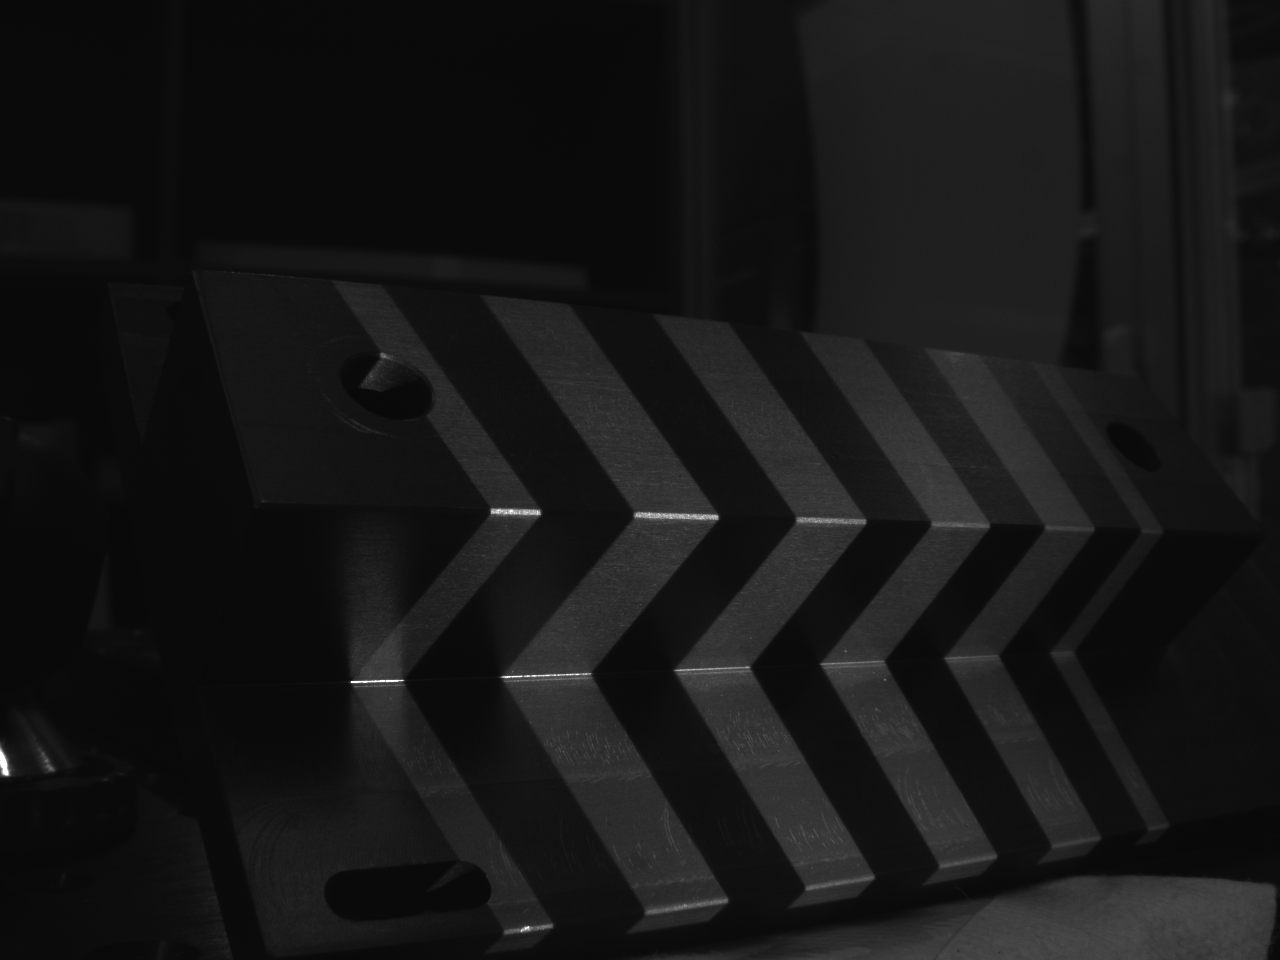
\includegraphics[width=0.49\linewidth]{images/snapshots_scan/SIMULATED-LEFT-LUMENERA-SN8010129/gray_05}
            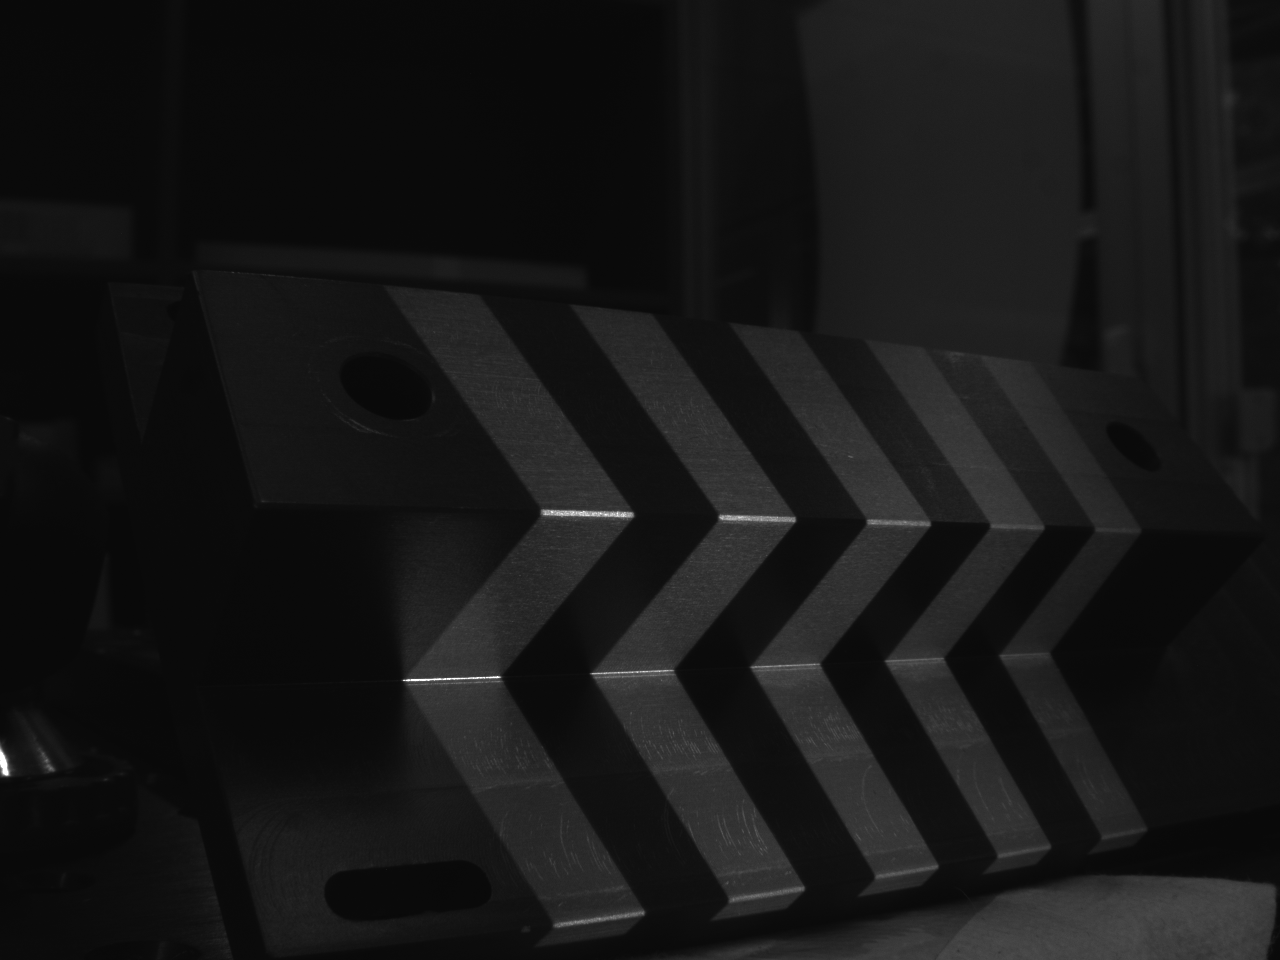
\includegraphics[width=0.49\linewidth]{images/snapshots_scan/SIMULATED-LEFT-LUMENERA-SN8010129/gray_05_inv}
        }
        \\
        \subfloat{
            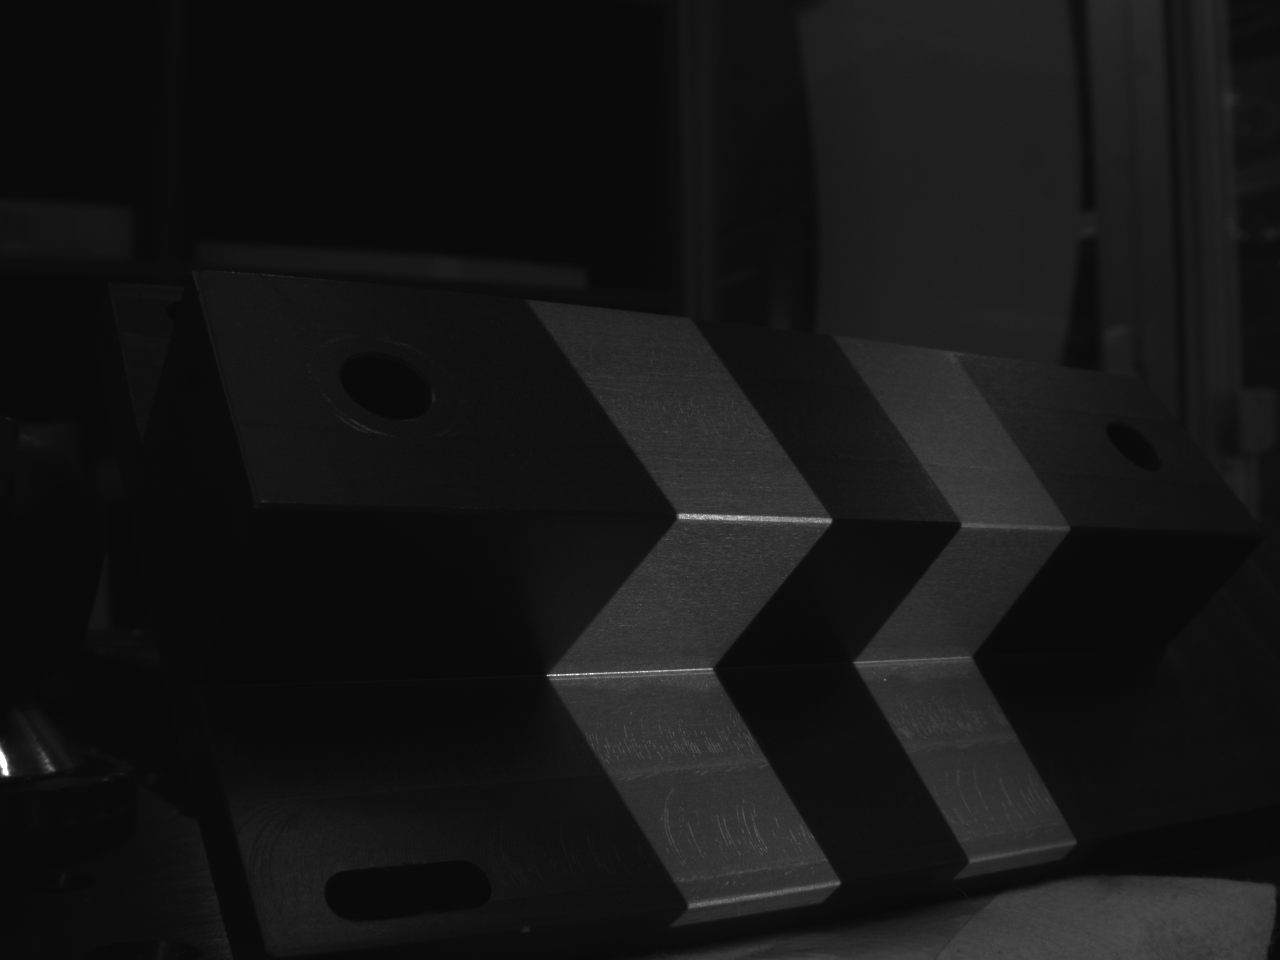
\includegraphics[width=0.49\linewidth]{images/snapshots_scan/SIMULATED-LEFT-LUMENERA-SN8010129/gray_06}
            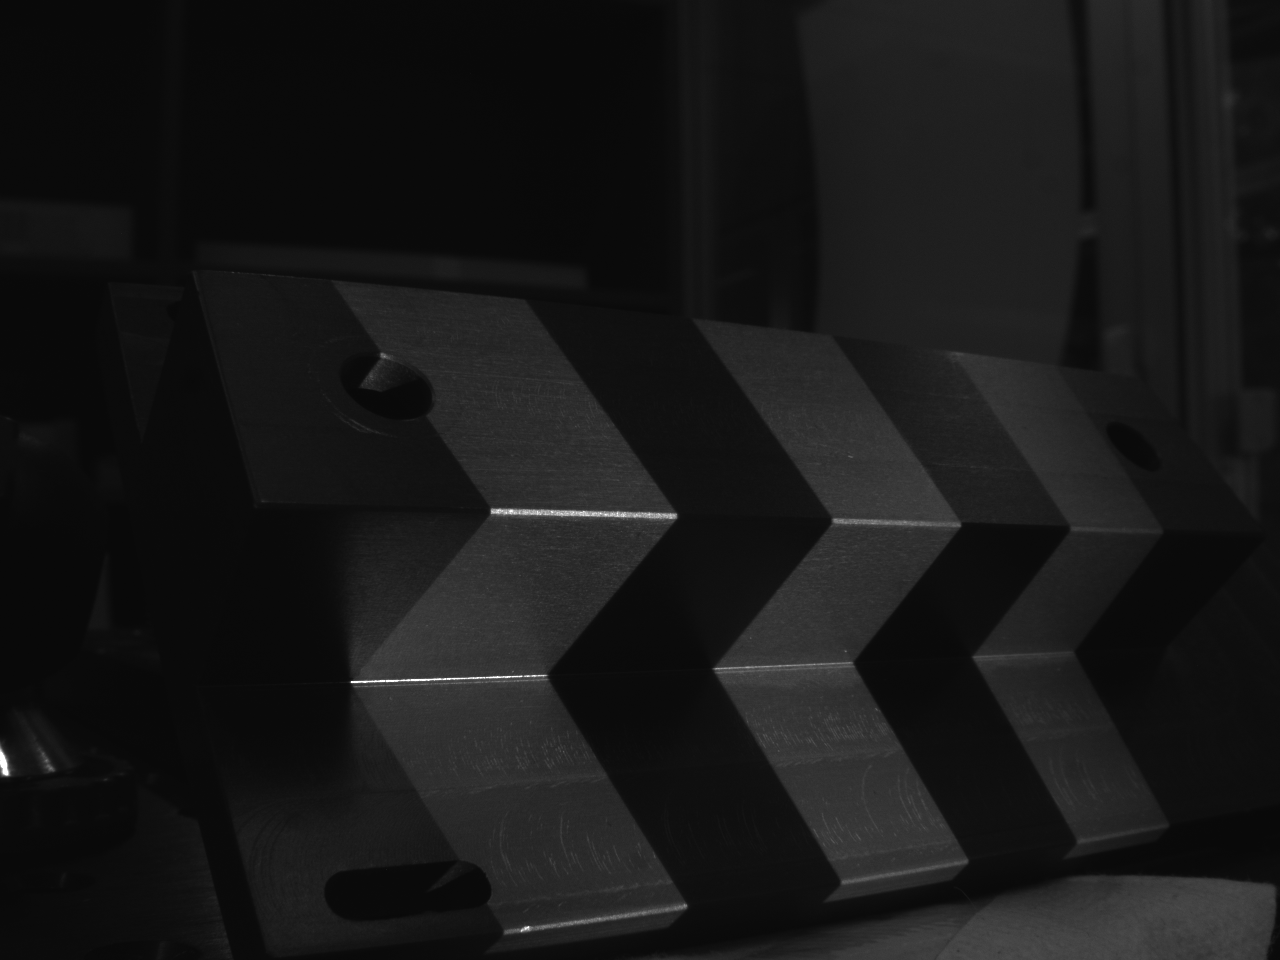
\includegraphics[width=0.49\linewidth]{images/snapshots_scan/SIMULATED-LEFT-LUMENERA-SN8010129/gray_06_inv}
        }
        \\
        \subfloat{
            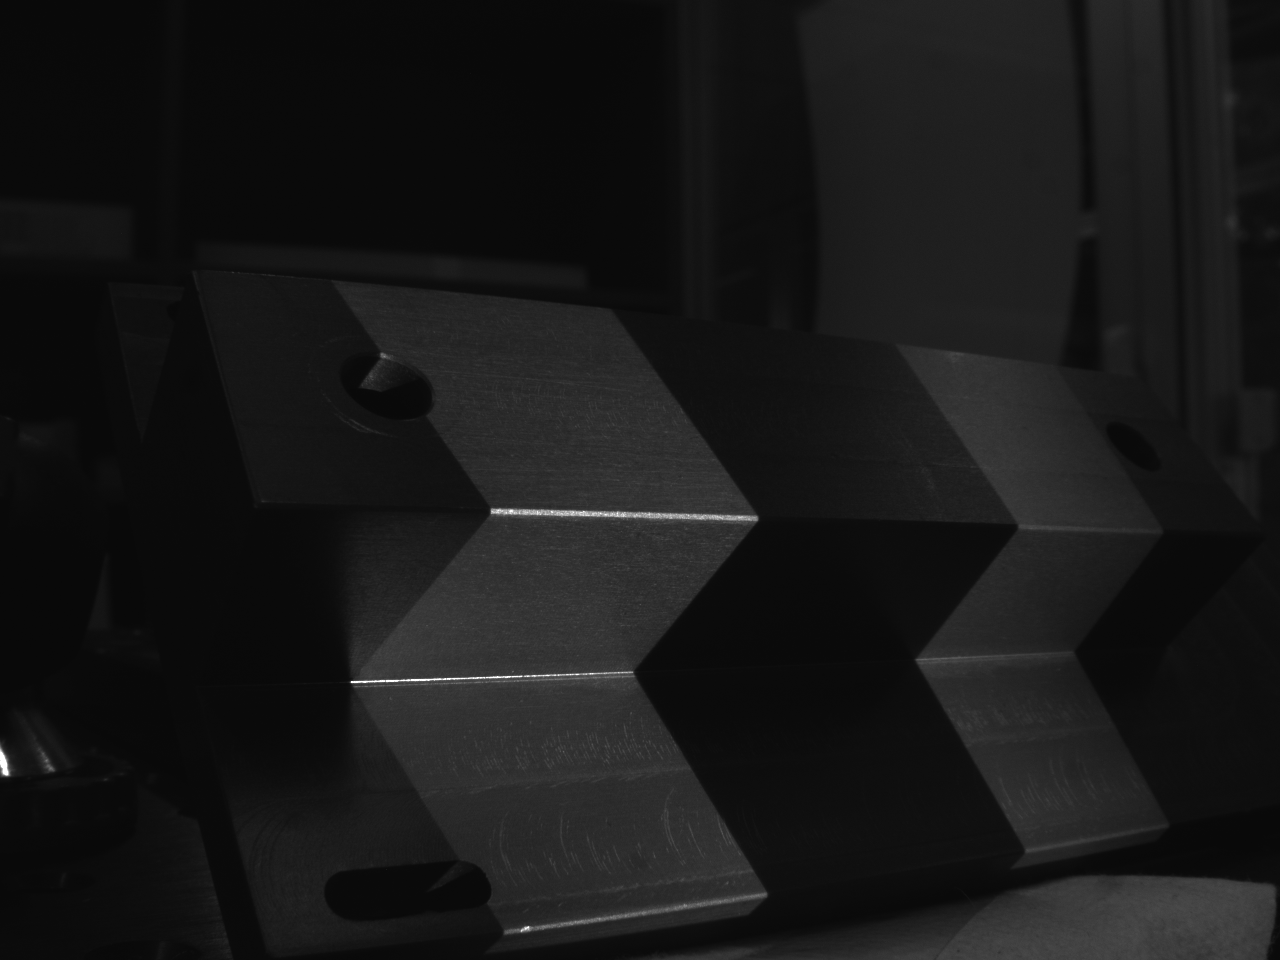
\includegraphics[width=0.49\linewidth]{images/snapshots_scan/SIMULATED-LEFT-LUMENERA-SN8010129/gray_07}
            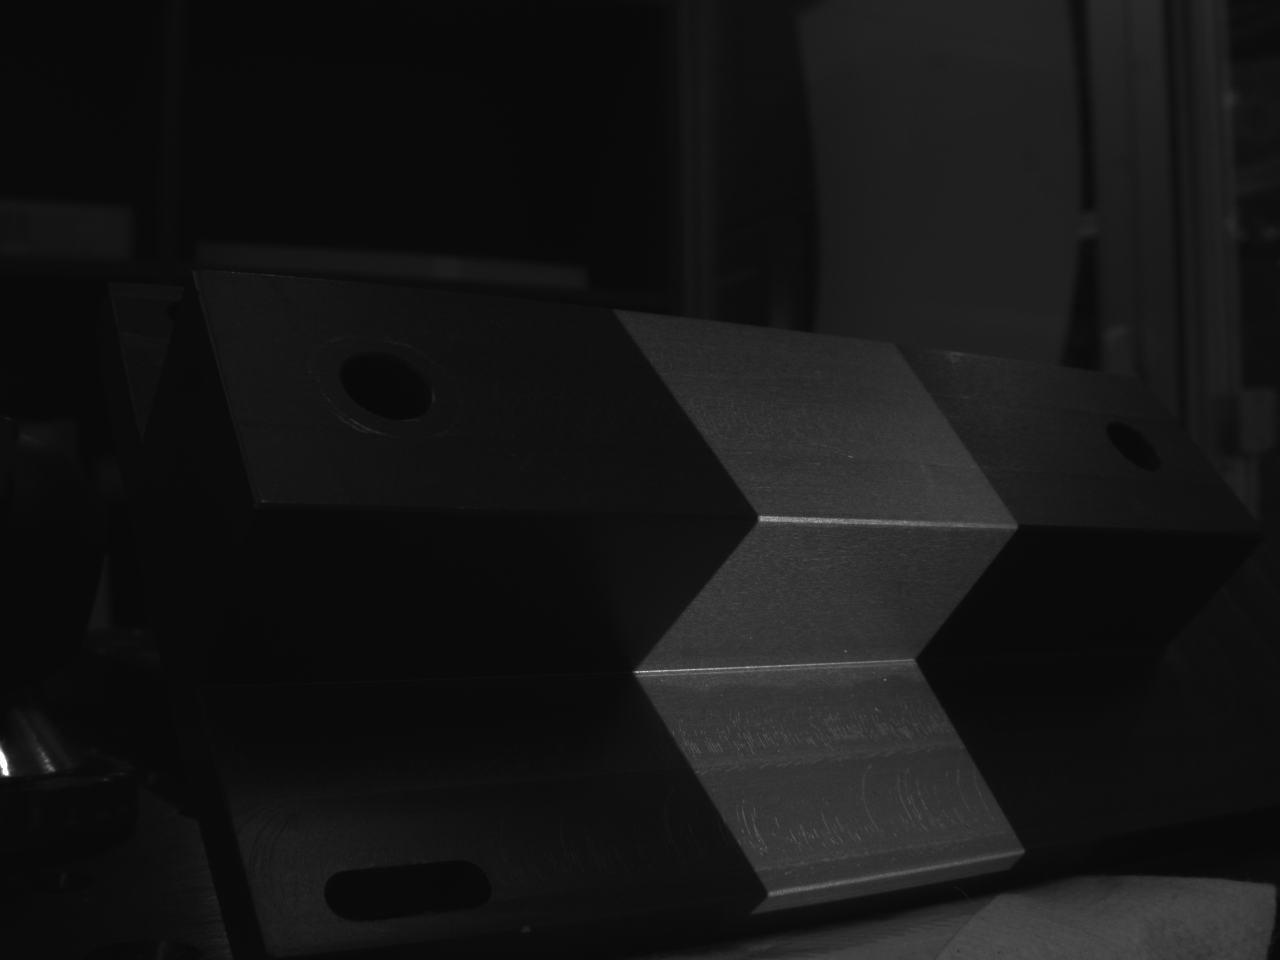
\includegraphics[width=0.49\linewidth]{images/snapshots_scan/SIMULATED-LEFT-LUMENERA-SN8010129/gray_07_inv}
        }
        \\
        \subfloat{
            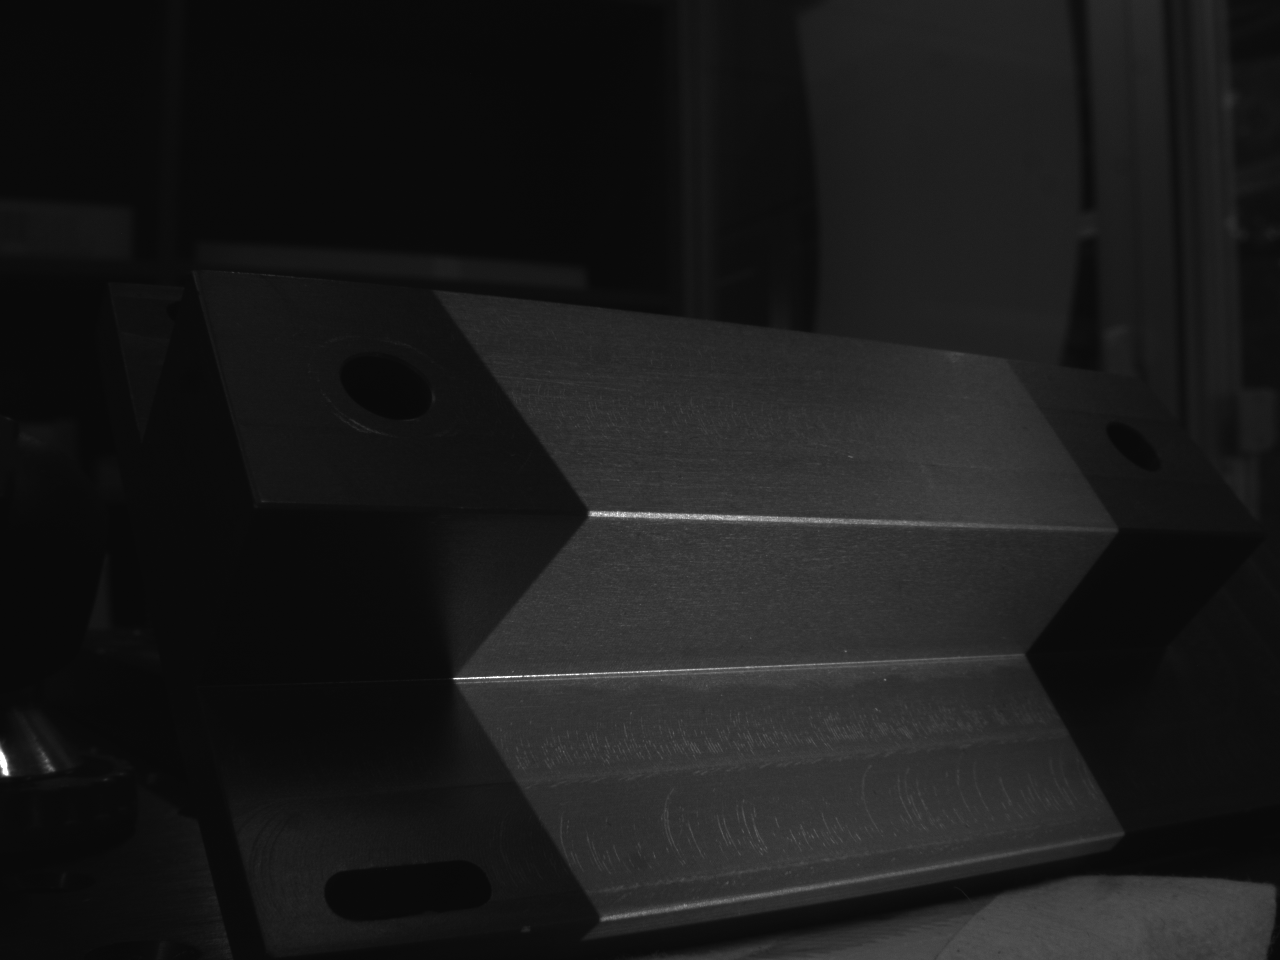
\includegraphics[width=0.49\linewidth]{images/snapshots_scan/SIMULATED-LEFT-LUMENERA-SN8010129/gray_08}
            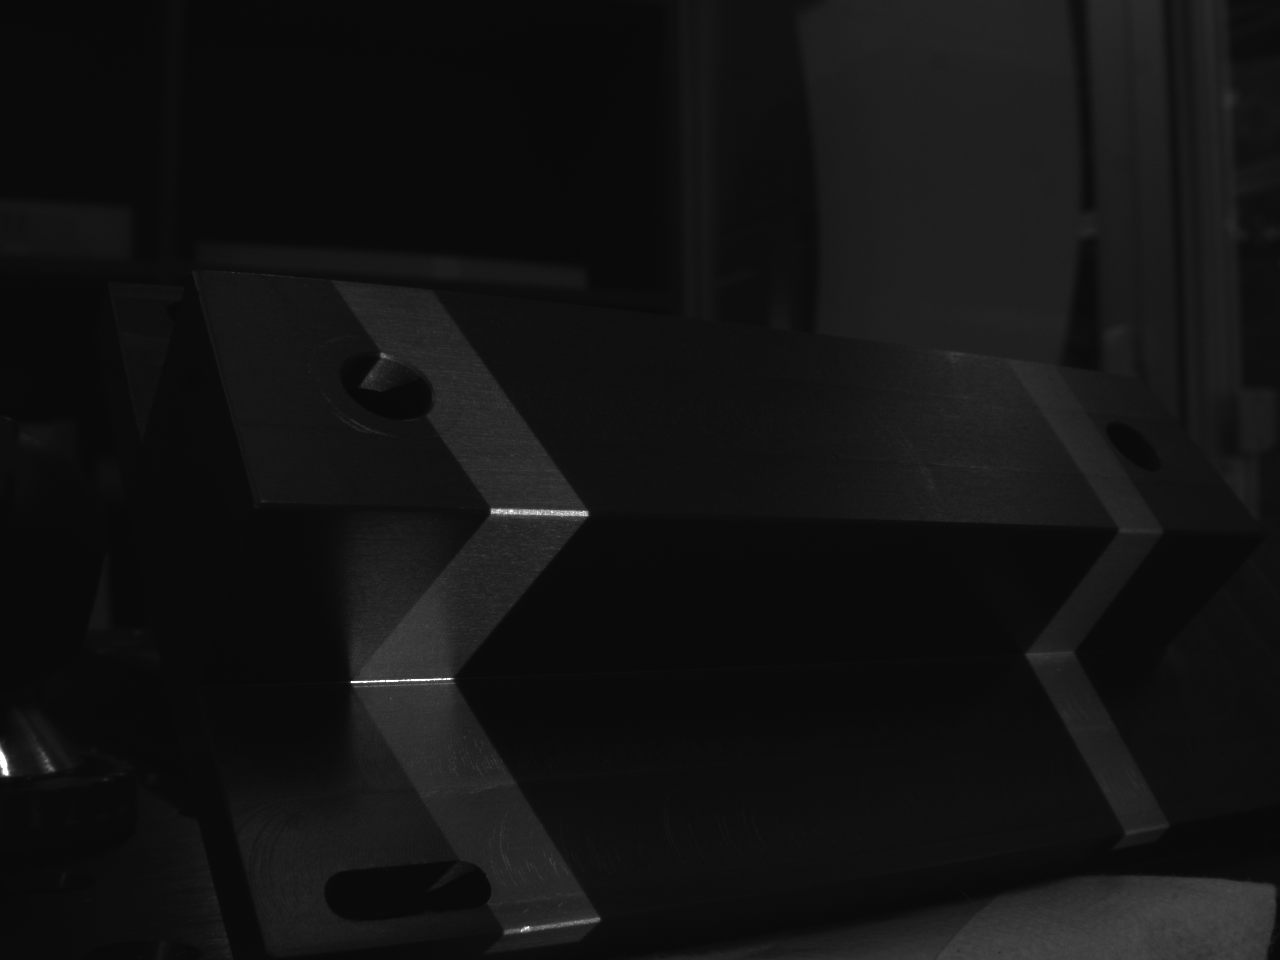
\includegraphics[width=0.49\linewidth]{images/snapshots_scan/SIMULATED-LEFT-LUMENERA-SN8010129/gray_08_inv}
        }
        \\
        \subfloat{
            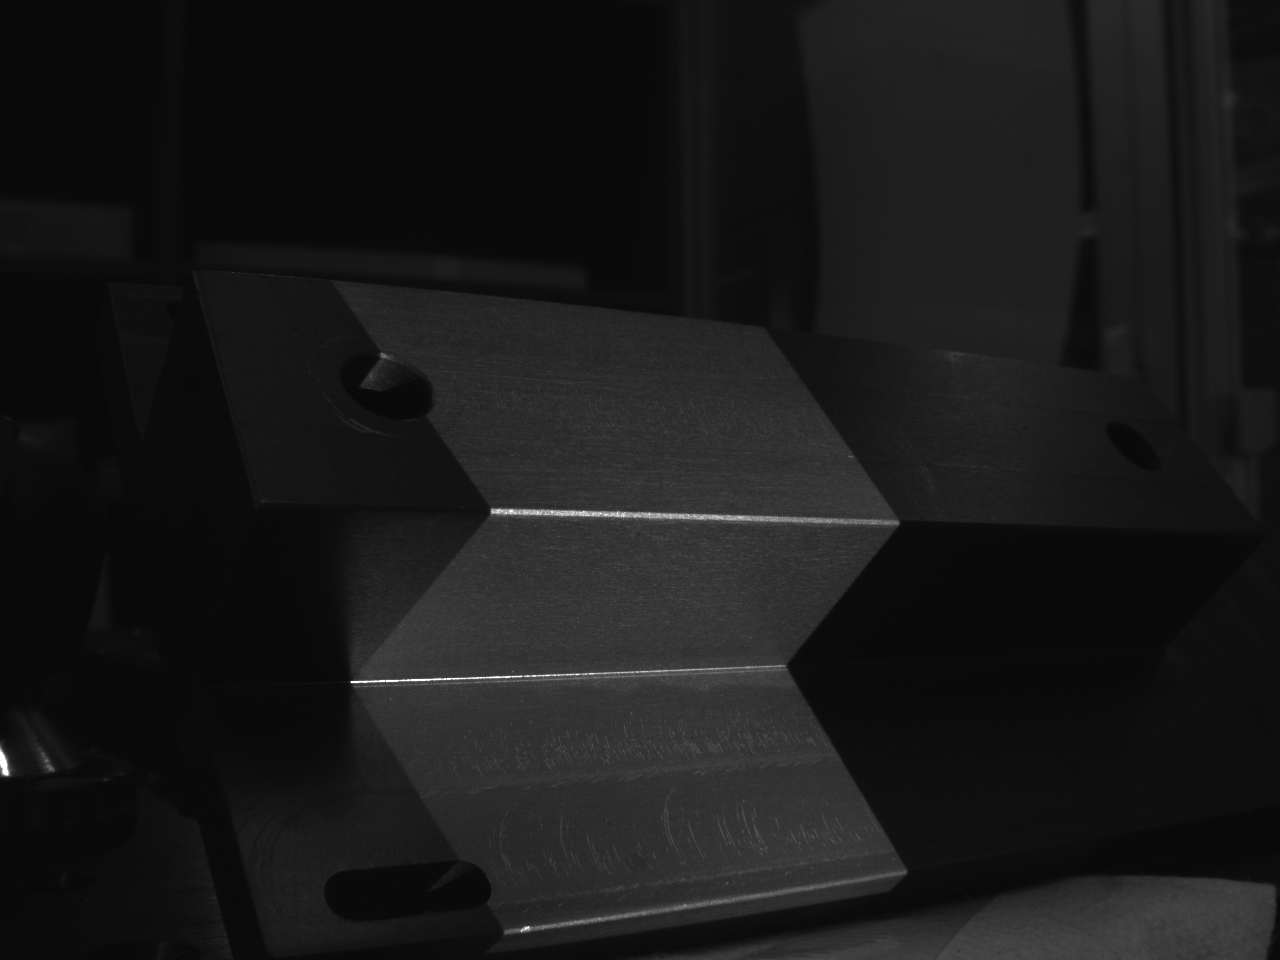
\includegraphics[width=0.49\linewidth]{images/snapshots_scan/SIMULATED-LEFT-LUMENERA-SN8010129/gray_09}
            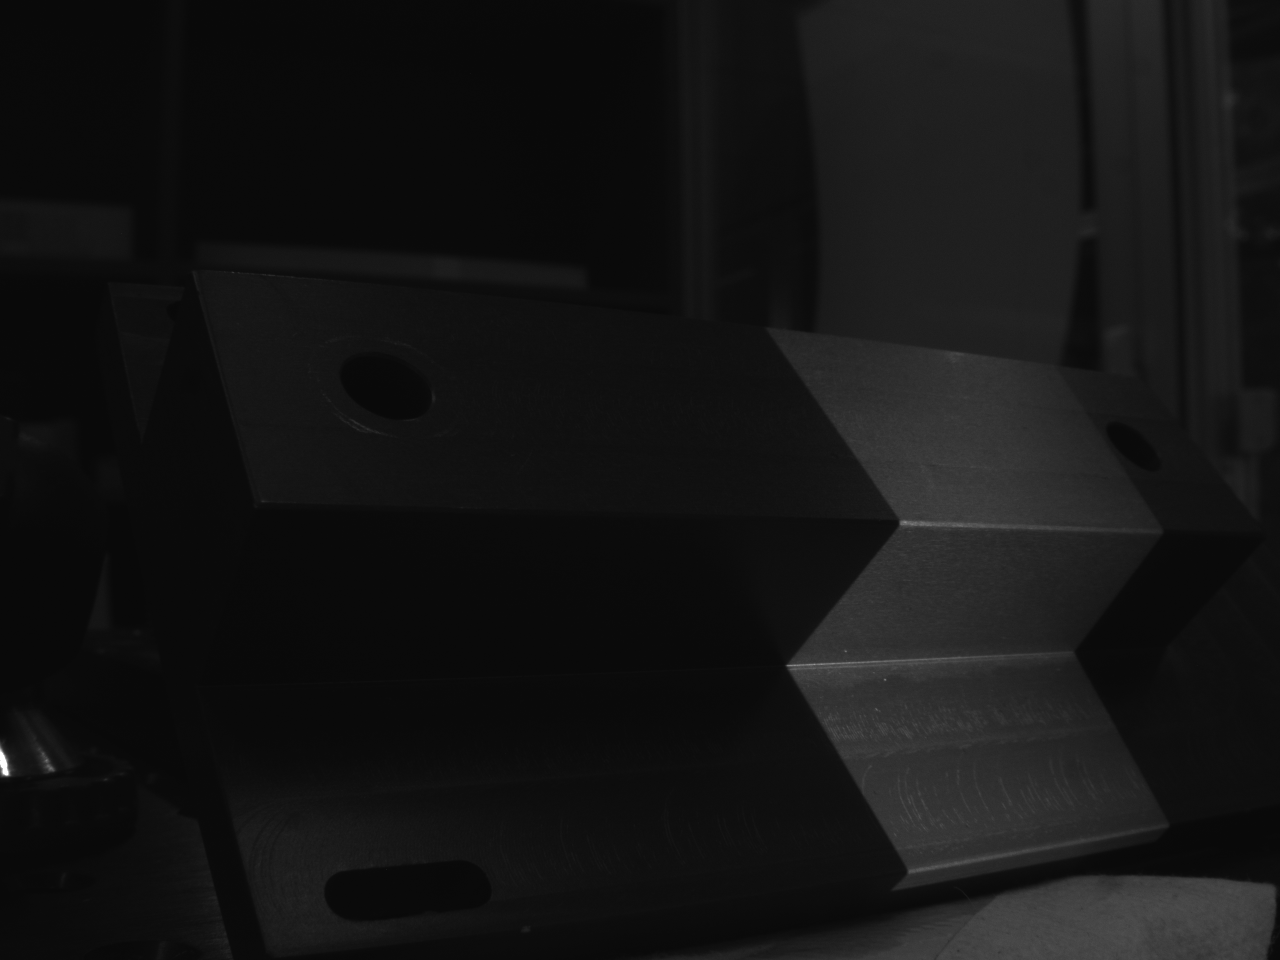
\includegraphics[width=0.49\linewidth]{images/snapshots_scan/SIMULATED-LEFT-LUMENERA-SN8010129/gray_09_inv}
        }
        \caption{Cámara izquierda: 5 últimos patrones proyectados (izq.) y su inverso (der.)}
        \label{fig:ejemploProyeccionCamaraIzquierda5a9}
\end{figure}

\begin{figure}[!bth]
    \myfloatalign
        \subfloat{
            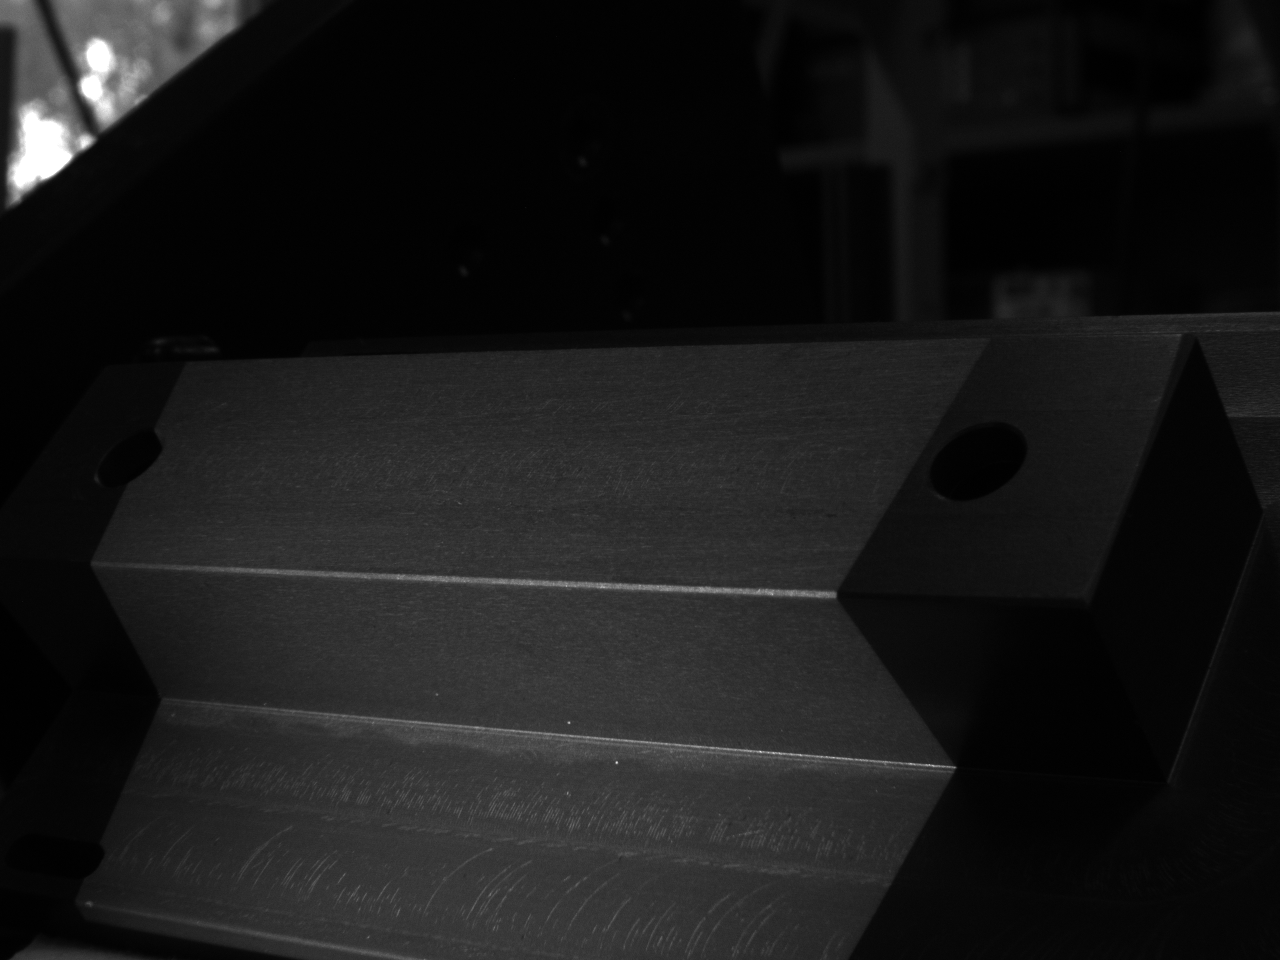
\includegraphics[width=0.49\linewidth]{images/snapshots_scan/SIMULATED-RIGHT-PGR-SN9041369/gray_00}
            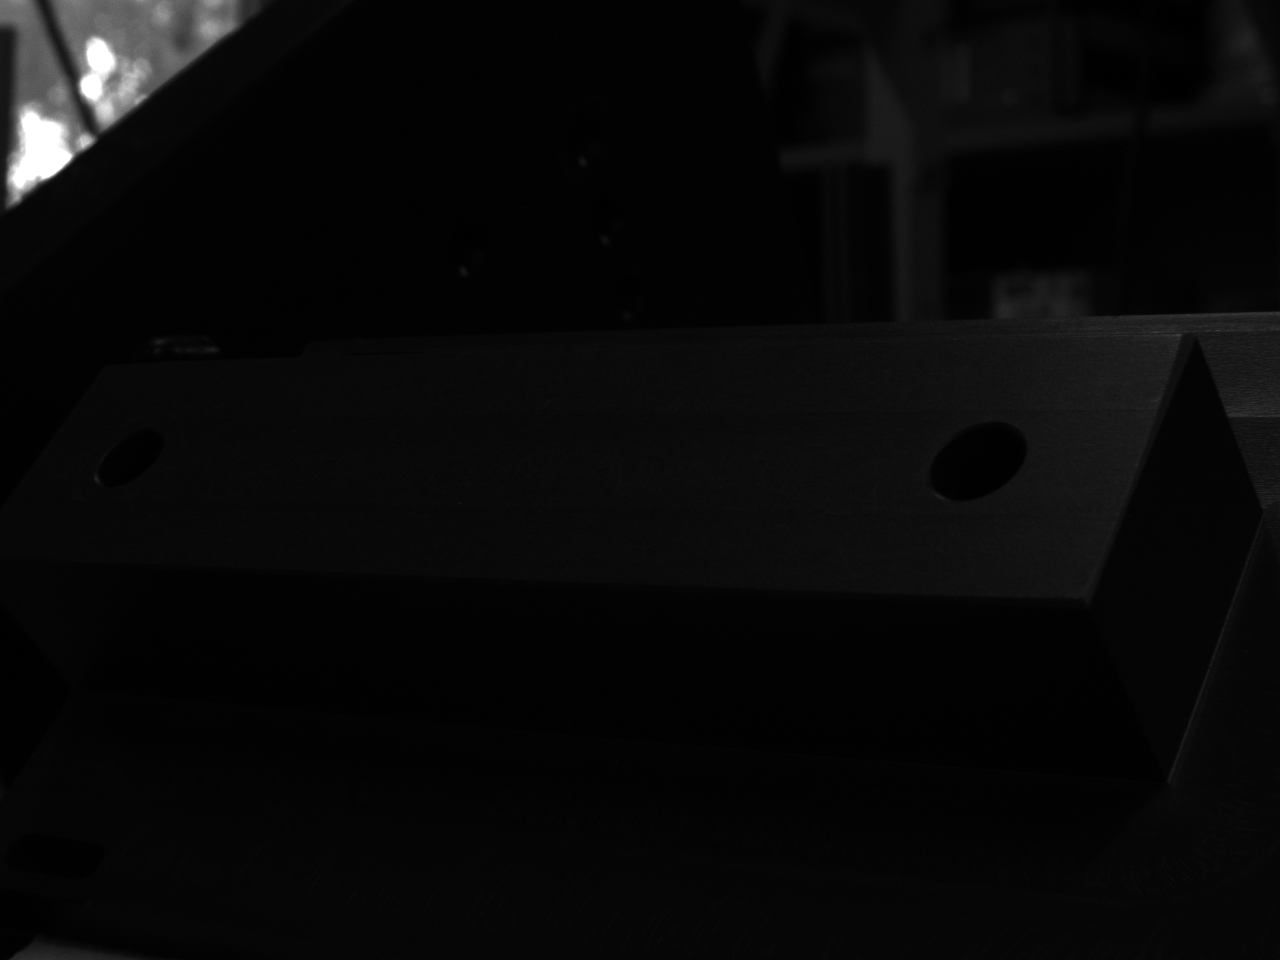
\includegraphics[width=0.49\linewidth]{images/snapshots_scan/SIMULATED-RIGHT-PGR-SN9041369/gray_00_inv}
        }
        \\
        \subfloat{
            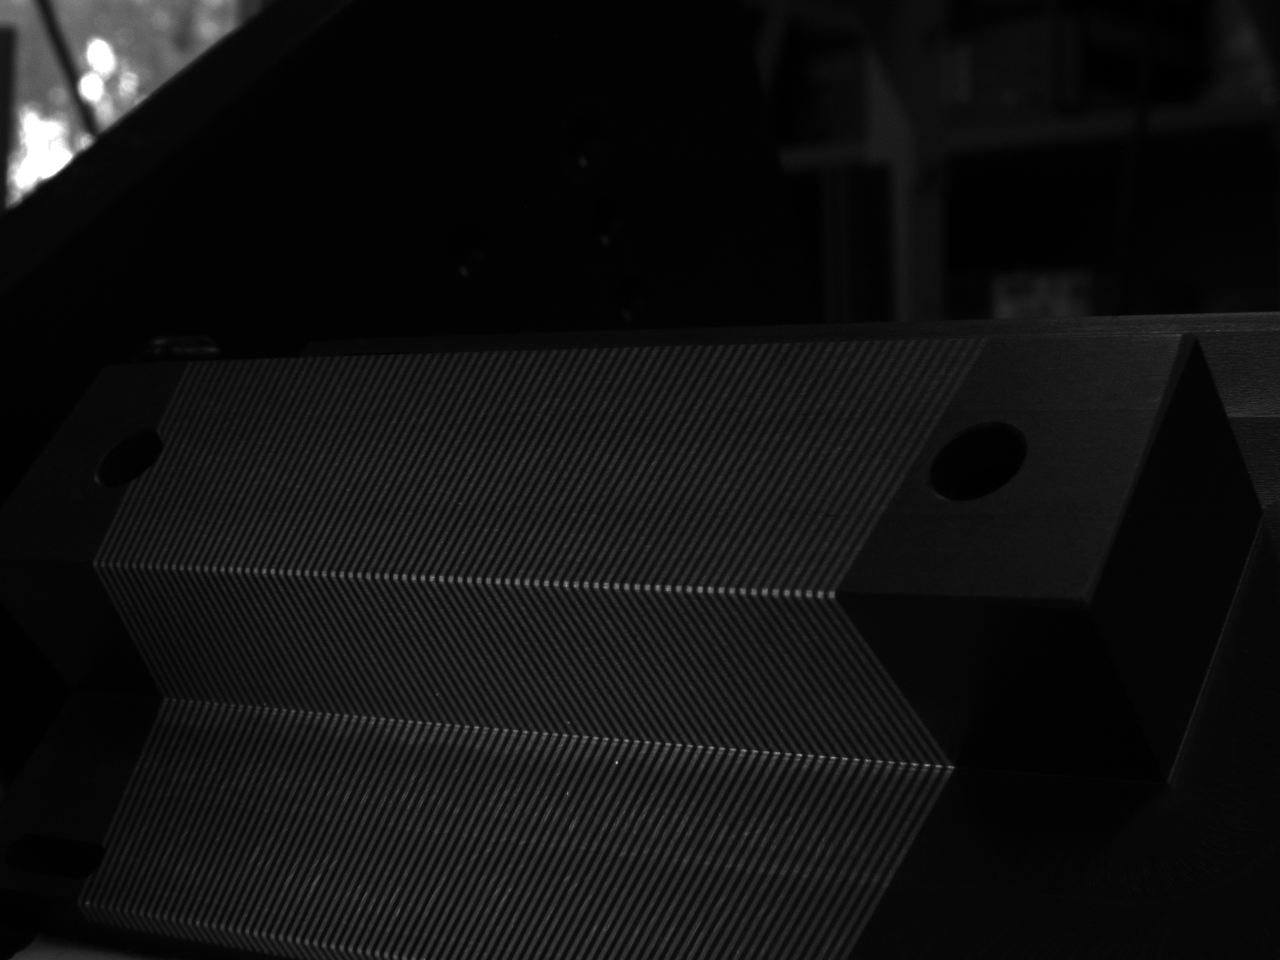
\includegraphics[width=0.49\linewidth]{images/snapshots_scan/SIMULATED-RIGHT-PGR-SN9041369/gray_01}
            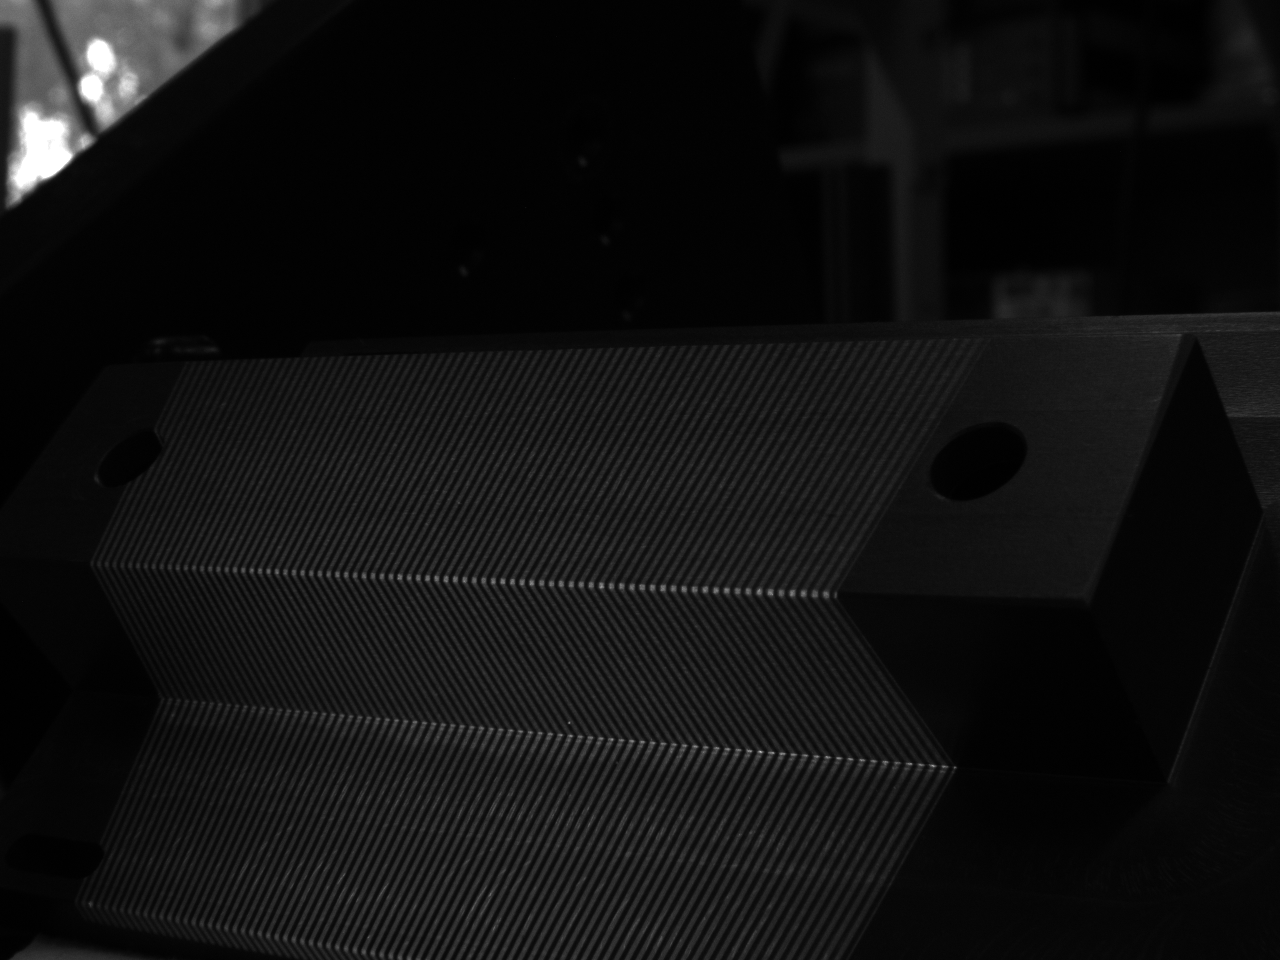
\includegraphics[width=0.49\linewidth]{images/snapshots_scan/SIMULATED-RIGHT-PGR-SN9041369/gray_01_inv}
        }
        \\
        \subfloat{
            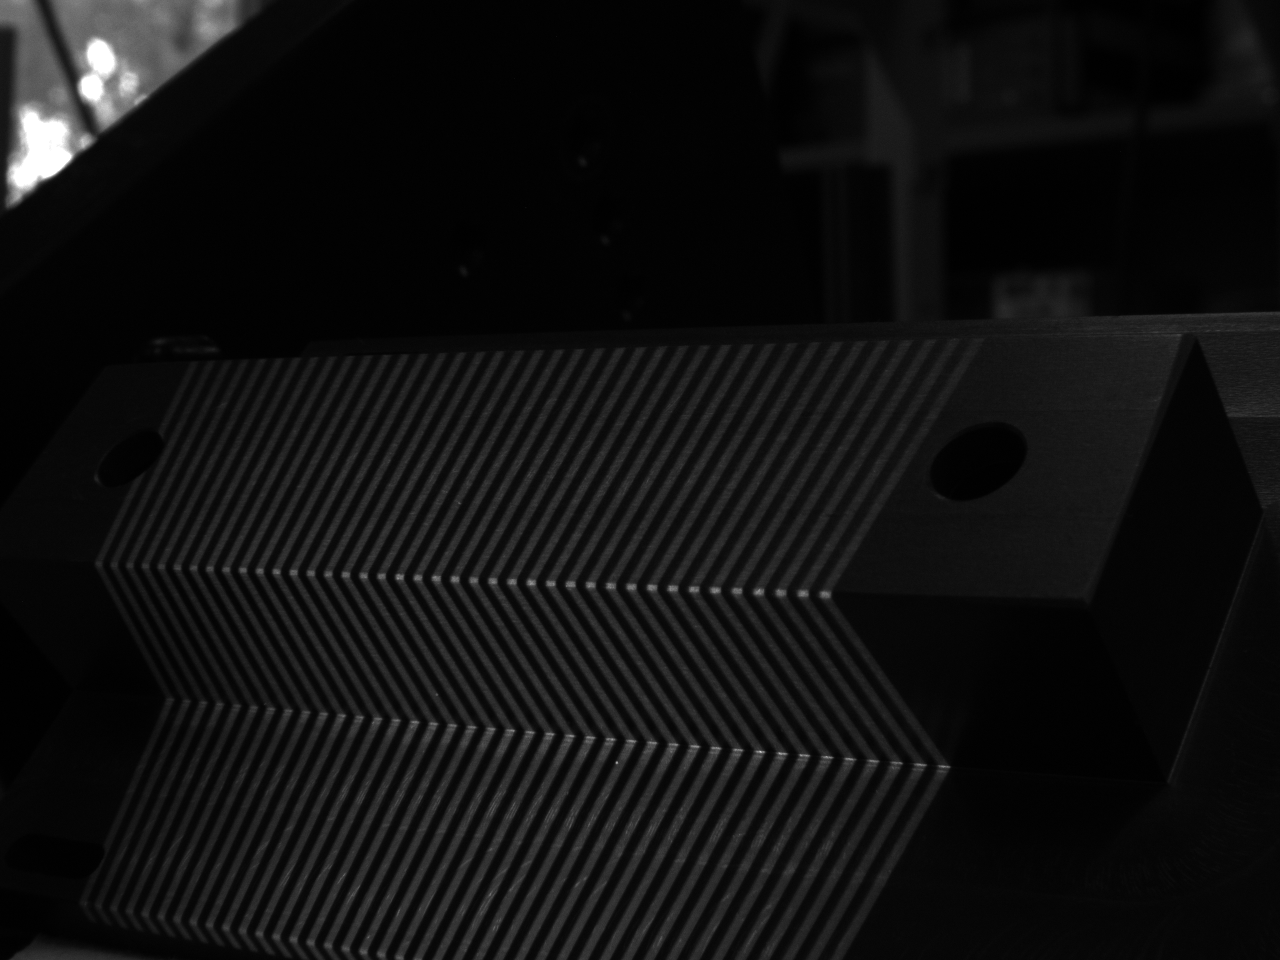
\includegraphics[width=0.49\linewidth]{images/snapshots_scan/SIMULATED-RIGHT-PGR-SN9041369/gray_02}
            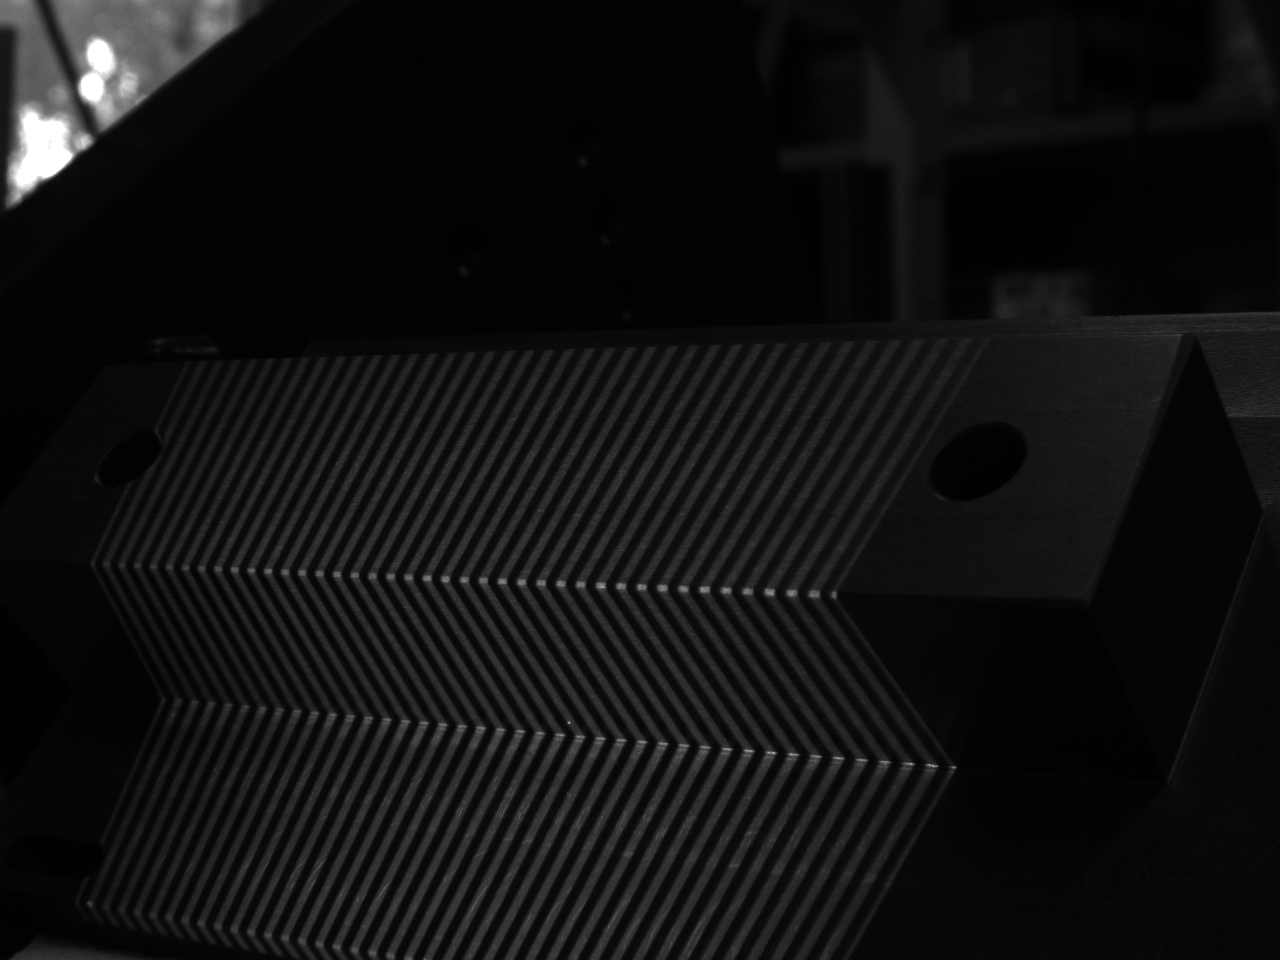
\includegraphics[width=0.49\linewidth]{images/snapshots_scan/SIMULATED-RIGHT-PGR-SN9041369/gray_02_inv}
        }
        \\
        \subfloat{
            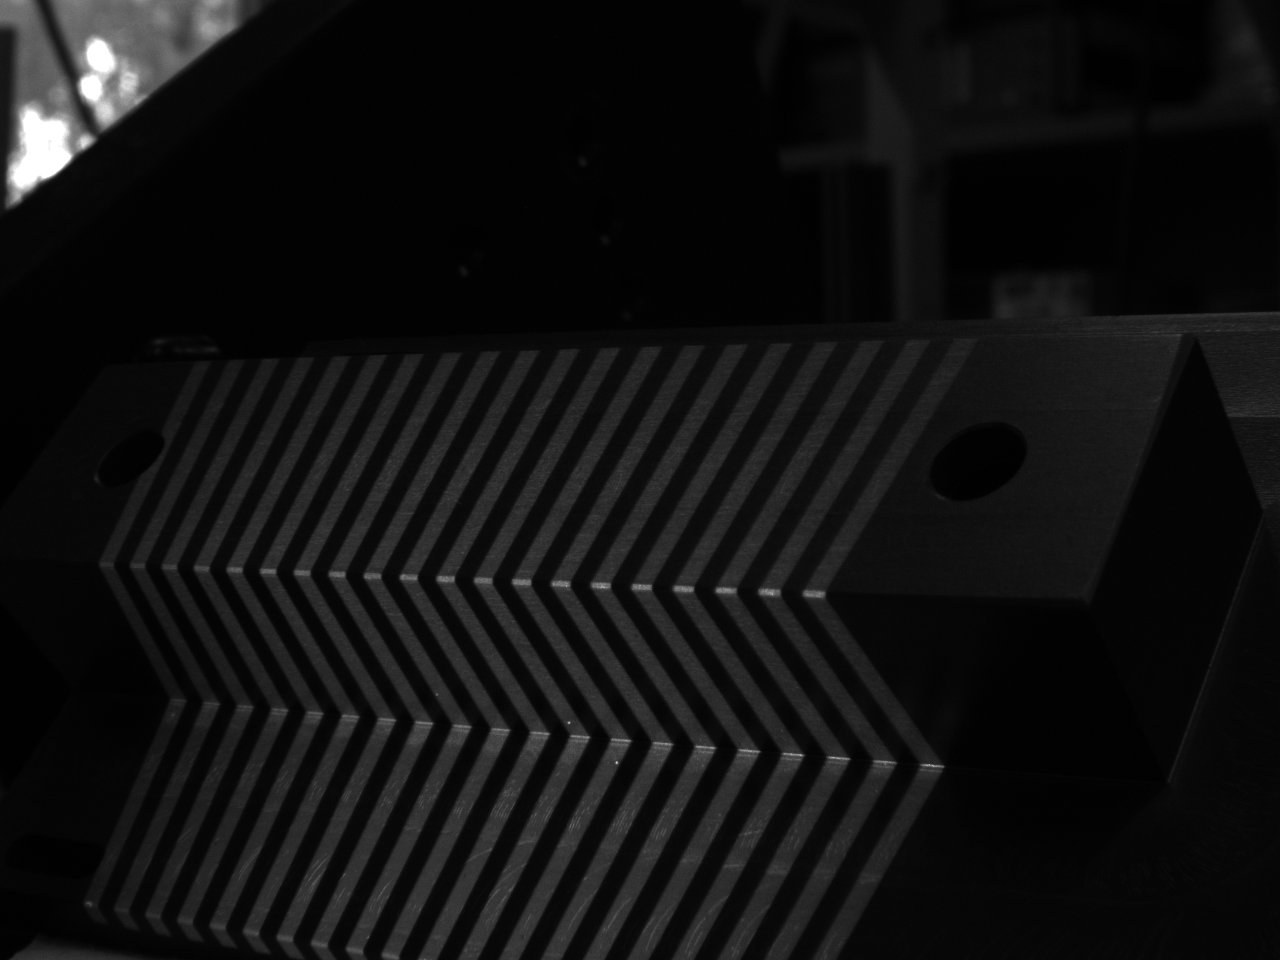
\includegraphics[width=0.49\linewidth]{images/snapshots_scan/SIMULATED-RIGHT-PGR-SN9041369/gray_03}
            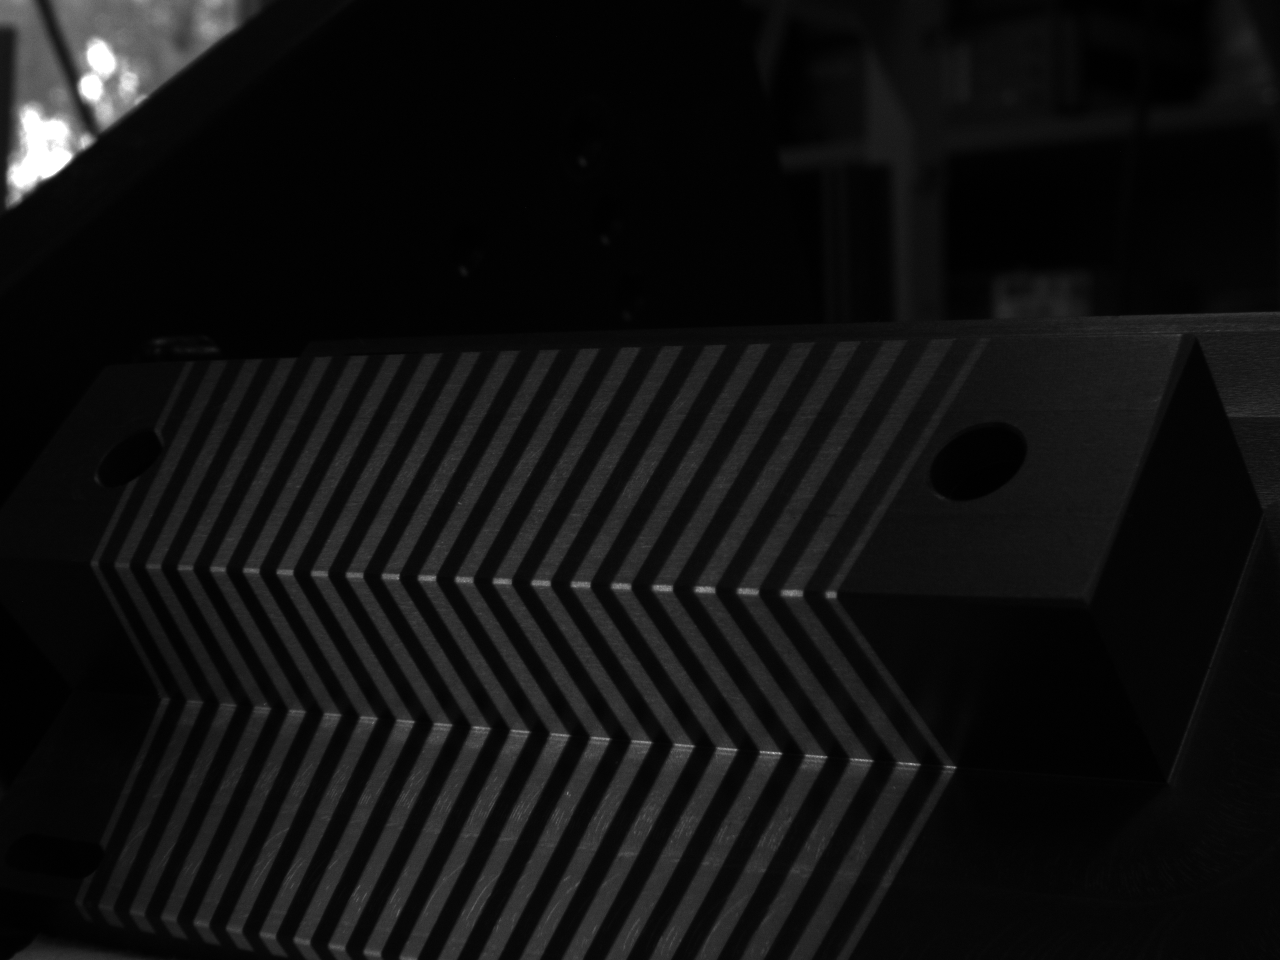
\includegraphics[width=0.49\linewidth]{images/snapshots_scan/SIMULATED-RIGHT-PGR-SN9041369/gray_03_inv}
        }
        \\
        \subfloat{
            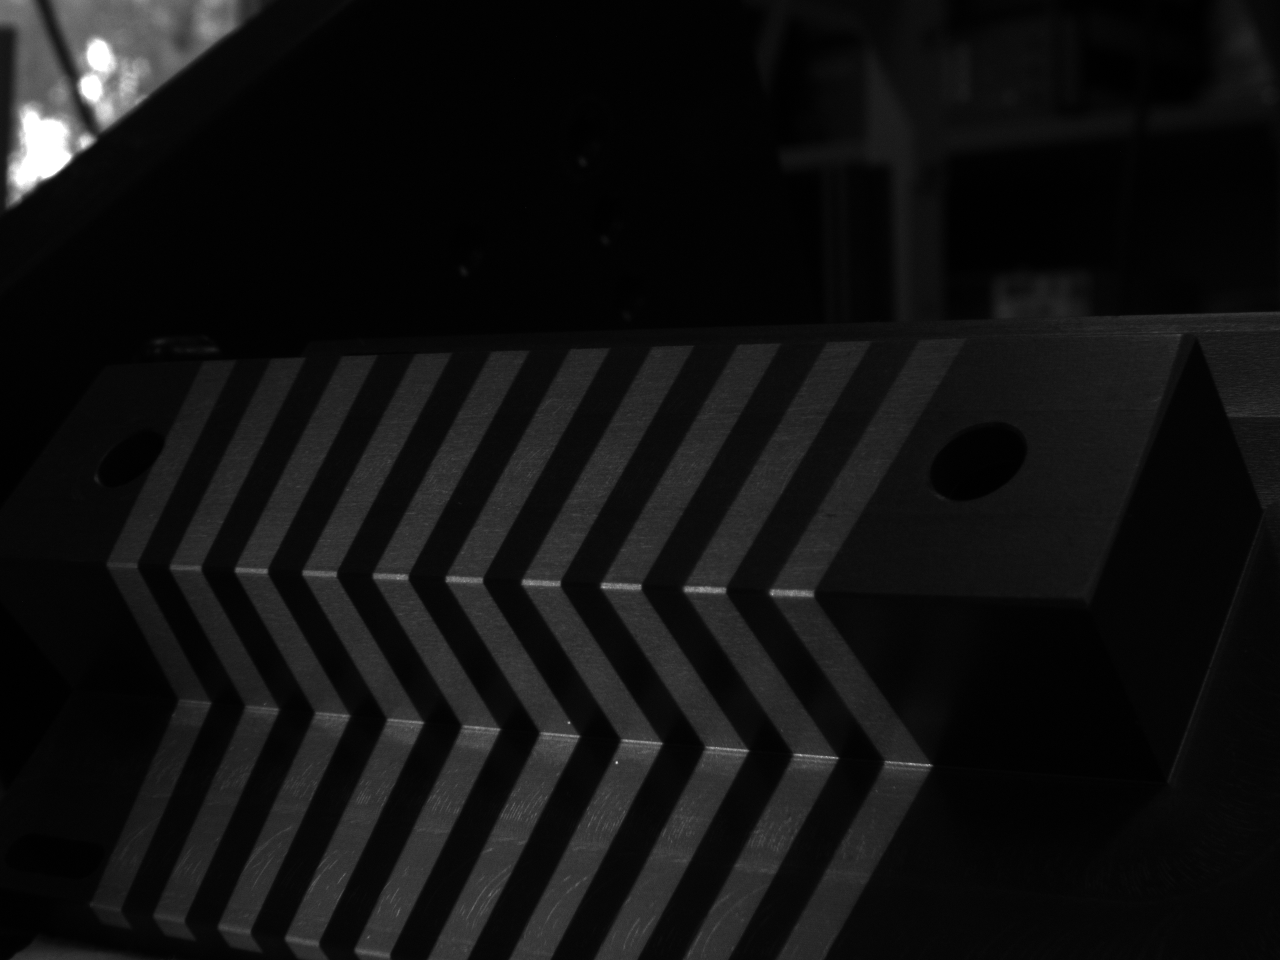
\includegraphics[width=0.49\linewidth]{images/snapshots_scan/SIMULATED-RIGHT-PGR-SN9041369/gray_04}
            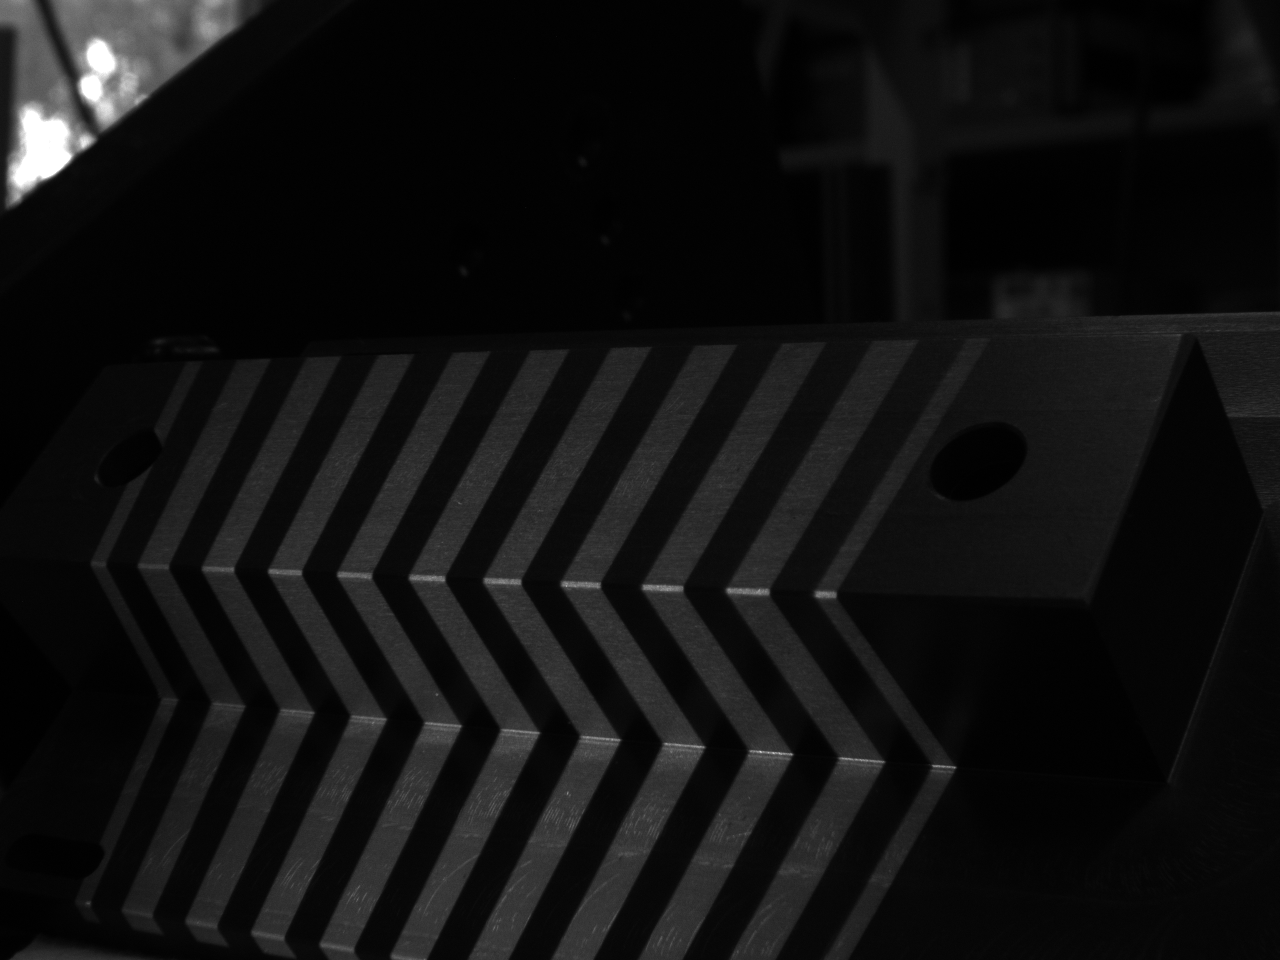
\includegraphics[width=0.49\linewidth]{images/snapshots_scan/SIMULATED-RIGHT-PGR-SN9041369/gray_04_inv}
        }
        \caption{Cámara derecha: 5 primeros patrones proyectados (izq.) y su inverso (der.)}
        \label{fig:ejemploProyeccionCamaraDerecha0a4}
\end{figure}

\begin{figure}[!bth]
    \myfloatalign
        \subfloat{
            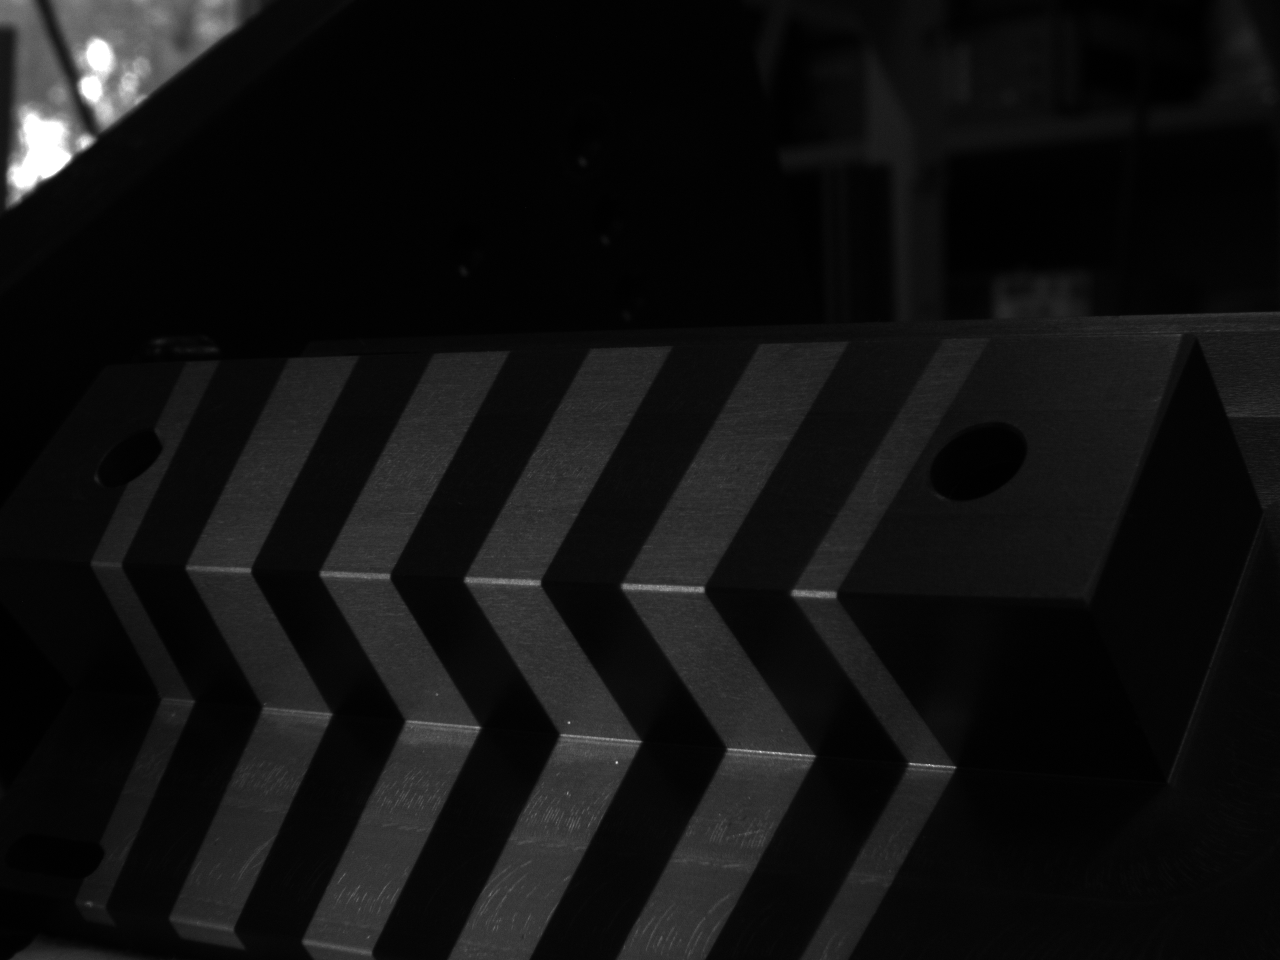
\includegraphics[width=0.49\linewidth]{images/snapshots_scan/SIMULATED-RIGHT-PGR-SN9041369/gray_05}
            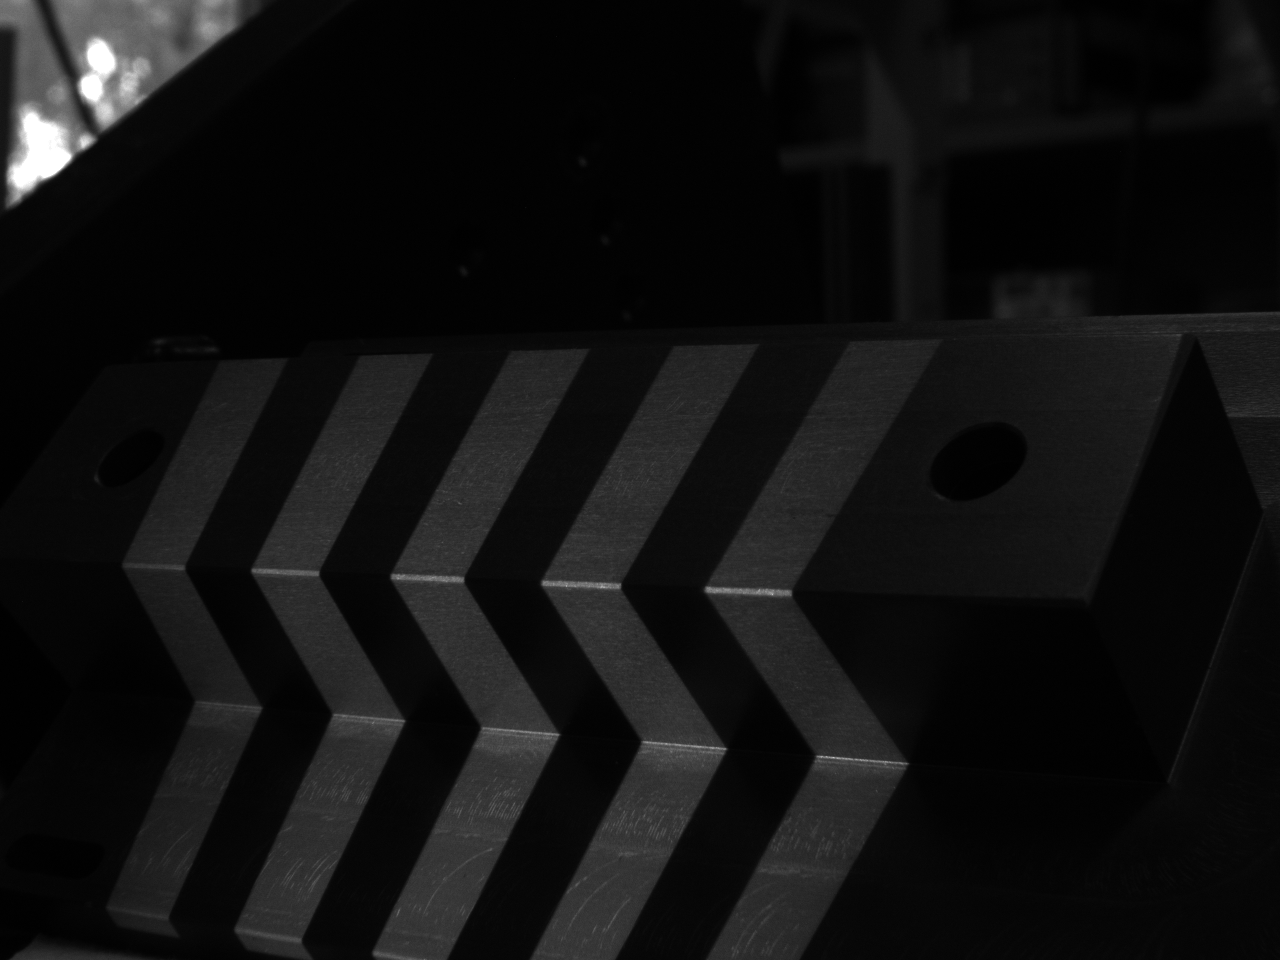
\includegraphics[width=0.49\linewidth]{images/snapshots_scan/SIMULATED-RIGHT-PGR-SN9041369/gray_05_inv}
        }
        \\
        \subfloat{
            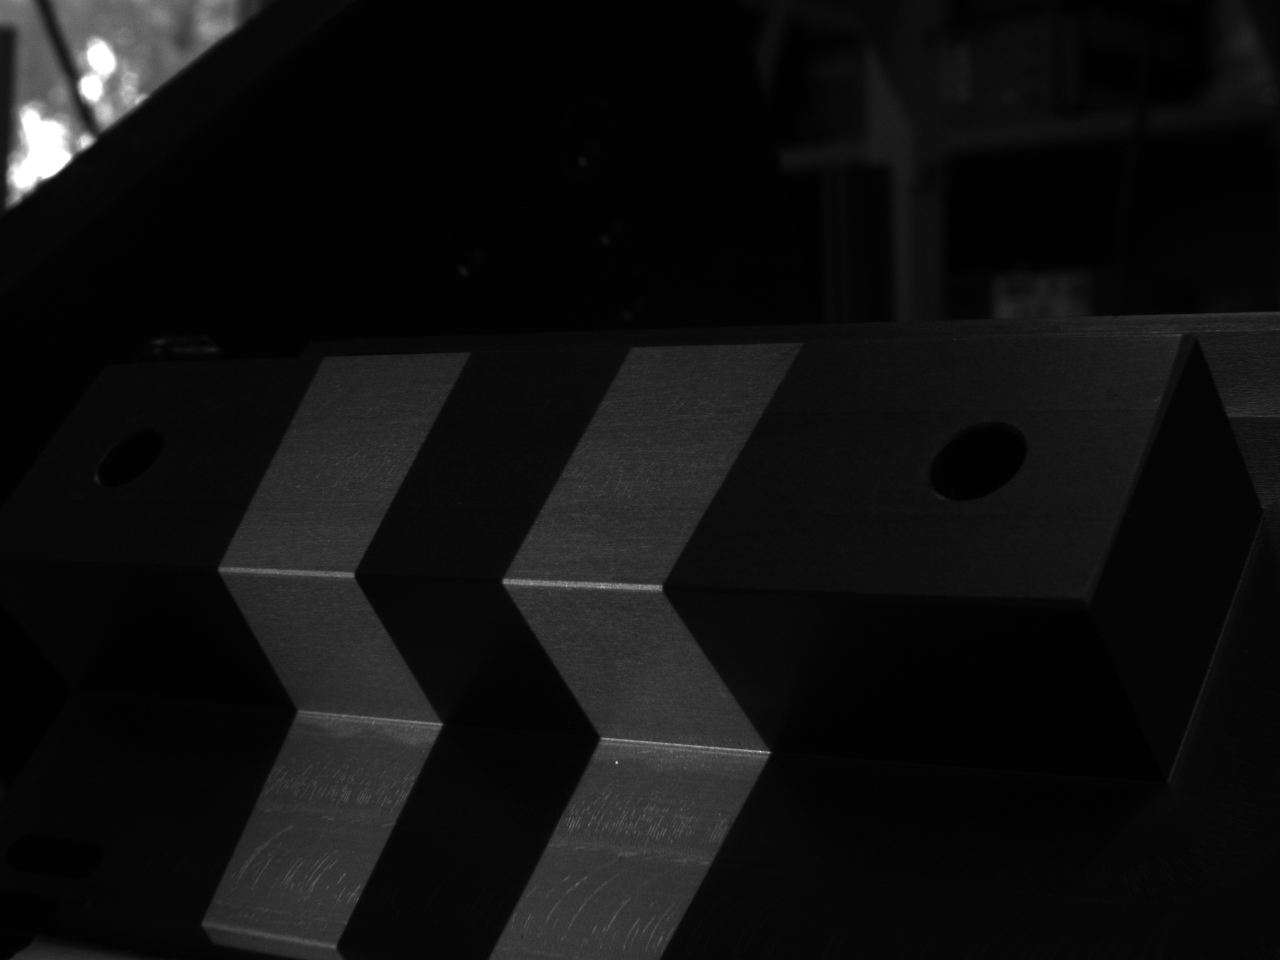
\includegraphics[width=0.49\linewidth]{images/snapshots_scan/SIMULATED-RIGHT-PGR-SN9041369/gray_06}
            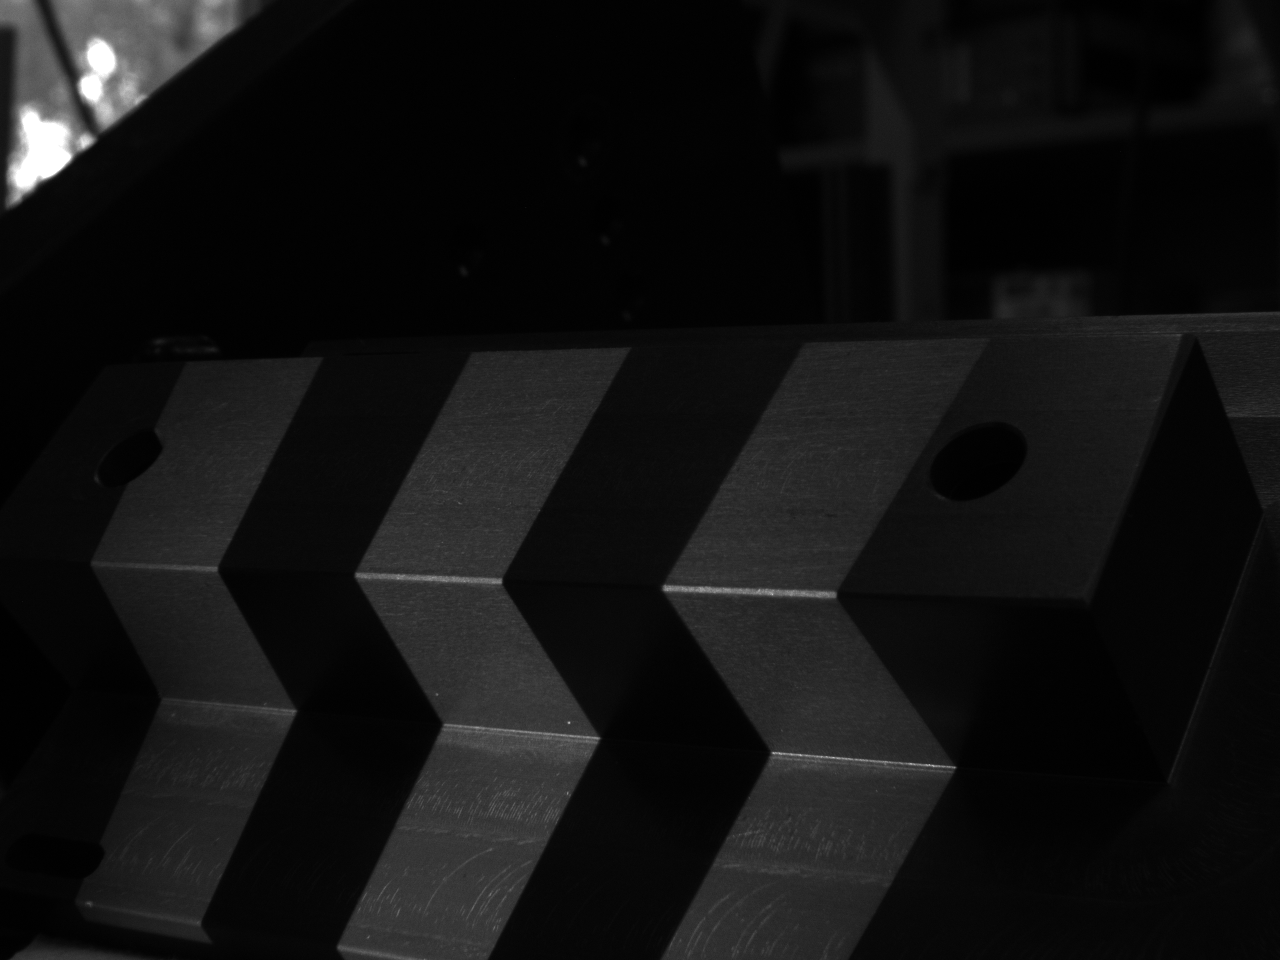
\includegraphics[width=0.49\linewidth]{images/snapshots_scan/SIMULATED-RIGHT-PGR-SN9041369/gray_06_inv}
        }
        \\
        \subfloat{
            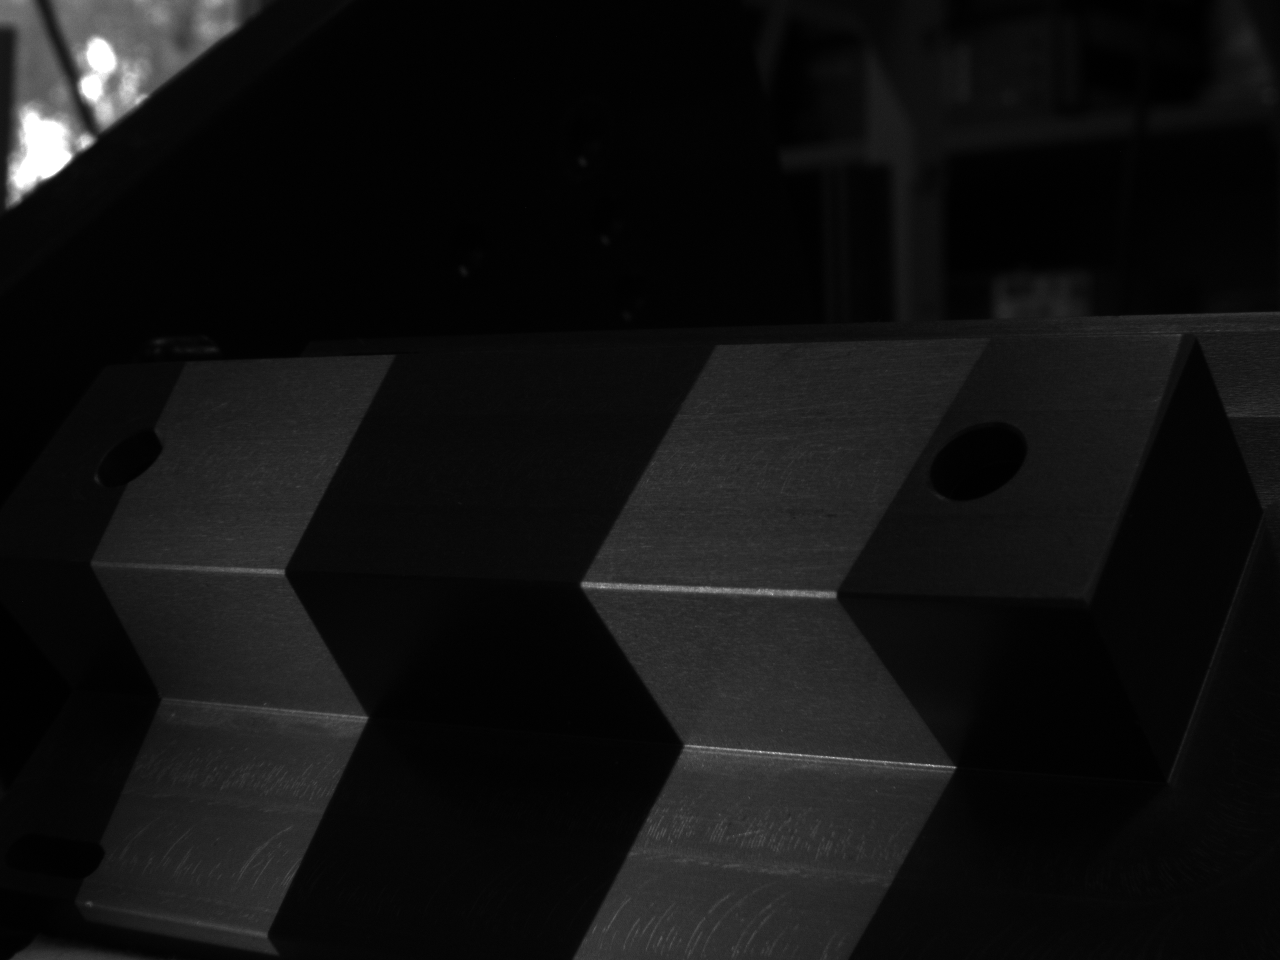
\includegraphics[width=0.49\linewidth]{images/snapshots_scan/SIMULATED-RIGHT-PGR-SN9041369/gray_07}
            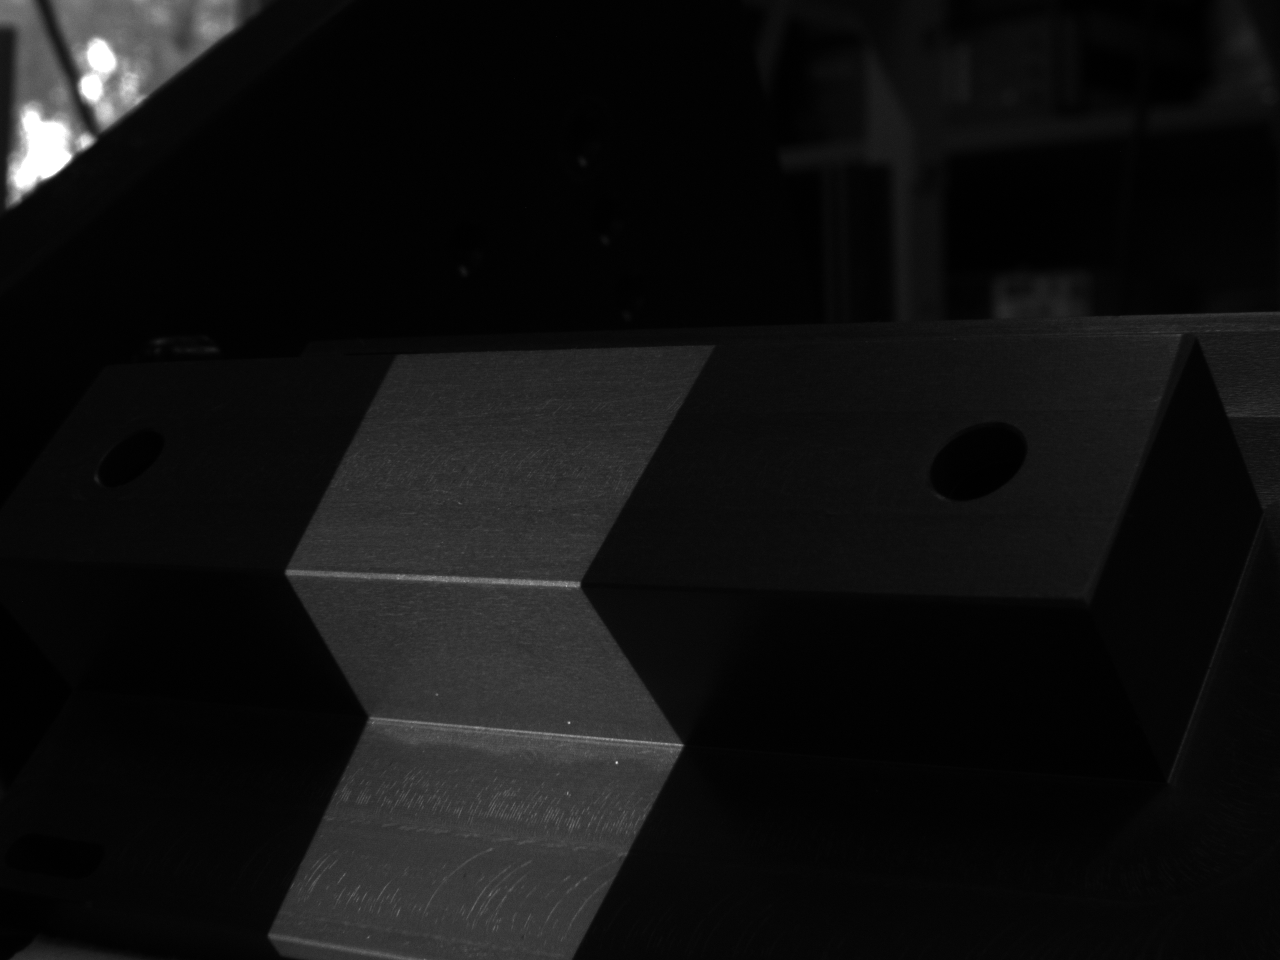
\includegraphics[width=0.49\linewidth]{images/snapshots_scan/SIMULATED-RIGHT-PGR-SN9041369/gray_07_inv}
        }
        \\
        \subfloat{
            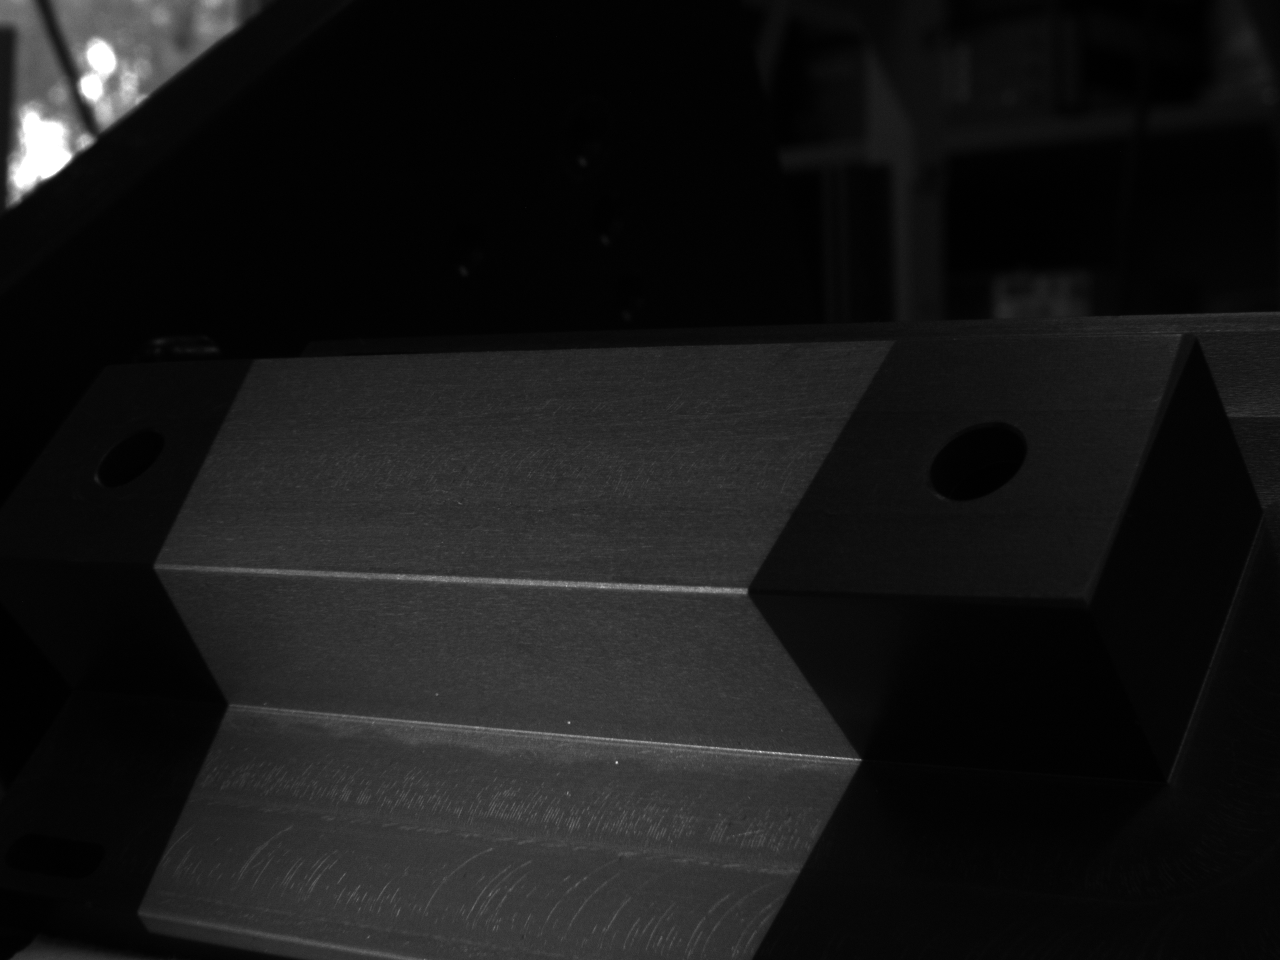
\includegraphics[width=0.49\linewidth]{images/snapshots_scan/SIMULATED-RIGHT-PGR-SN9041369/gray_08}
            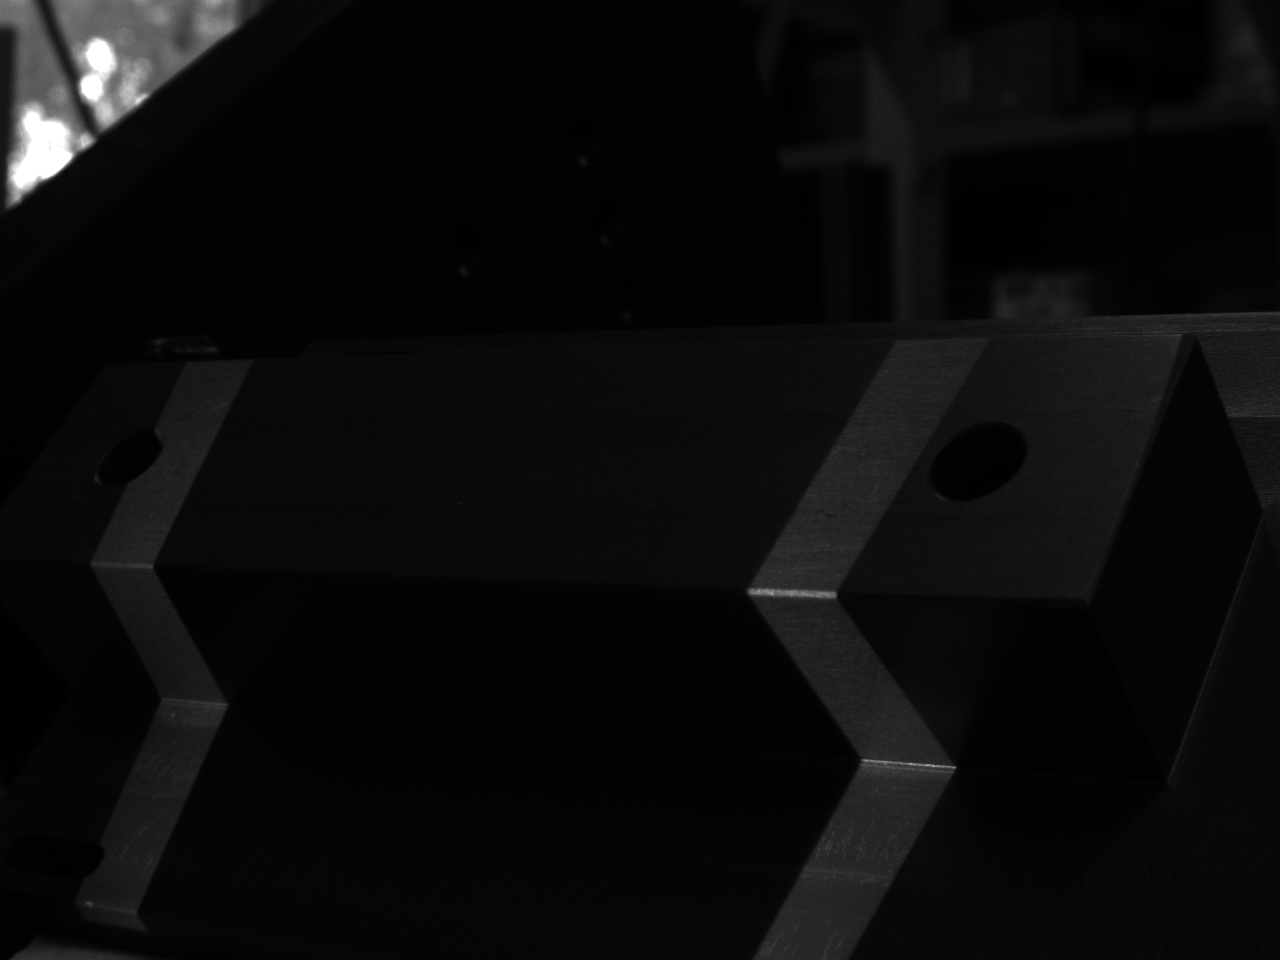
\includegraphics[width=0.49\linewidth]{images/snapshots_scan/SIMULATED-RIGHT-PGR-SN9041369/gray_08_inv}
        }
        \\
        \subfloat{
            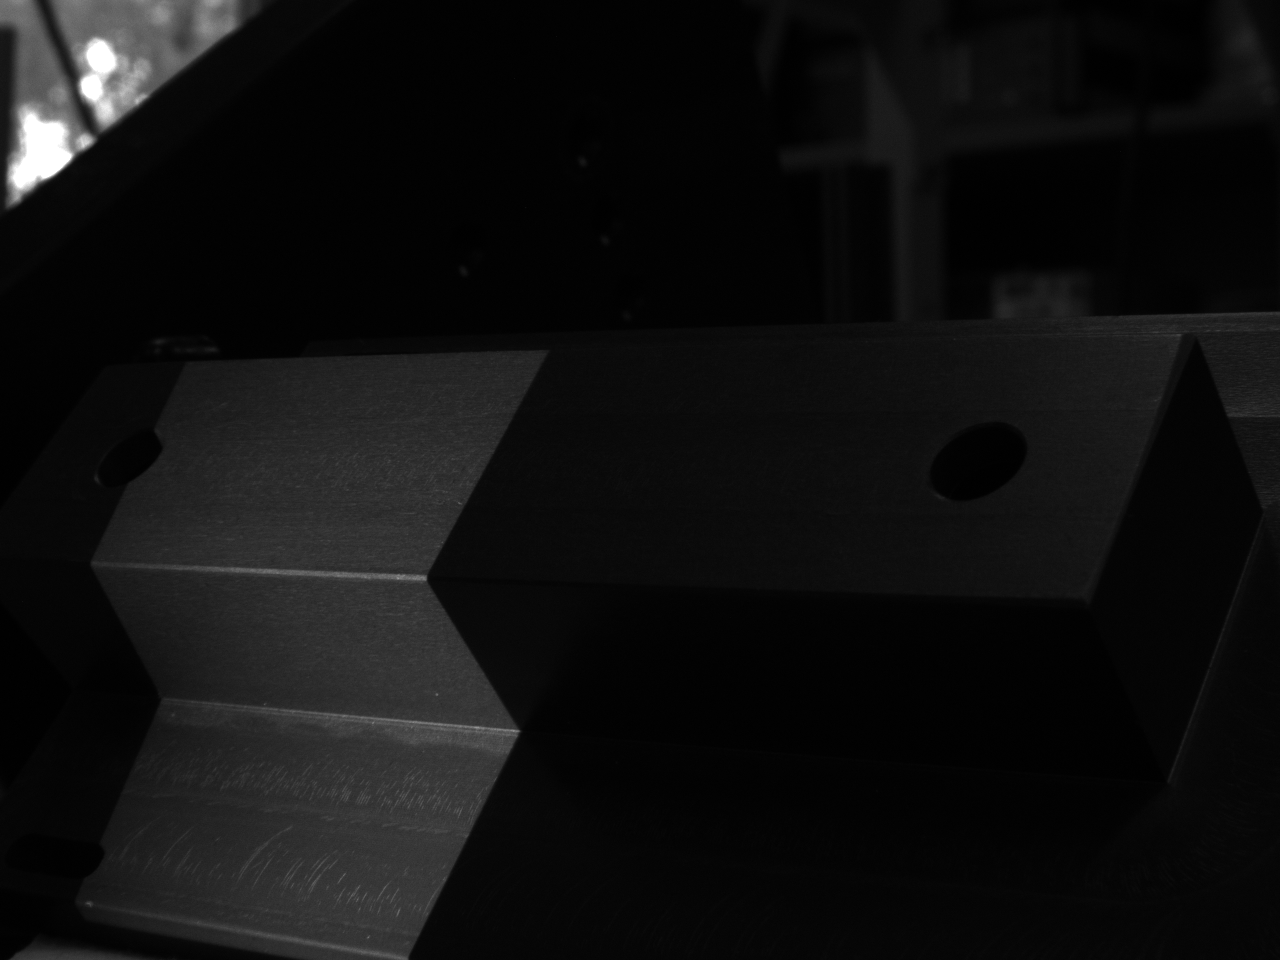
\includegraphics[width=0.49\linewidth]{images/snapshots_scan/SIMULATED-RIGHT-PGR-SN9041369/gray_09}
            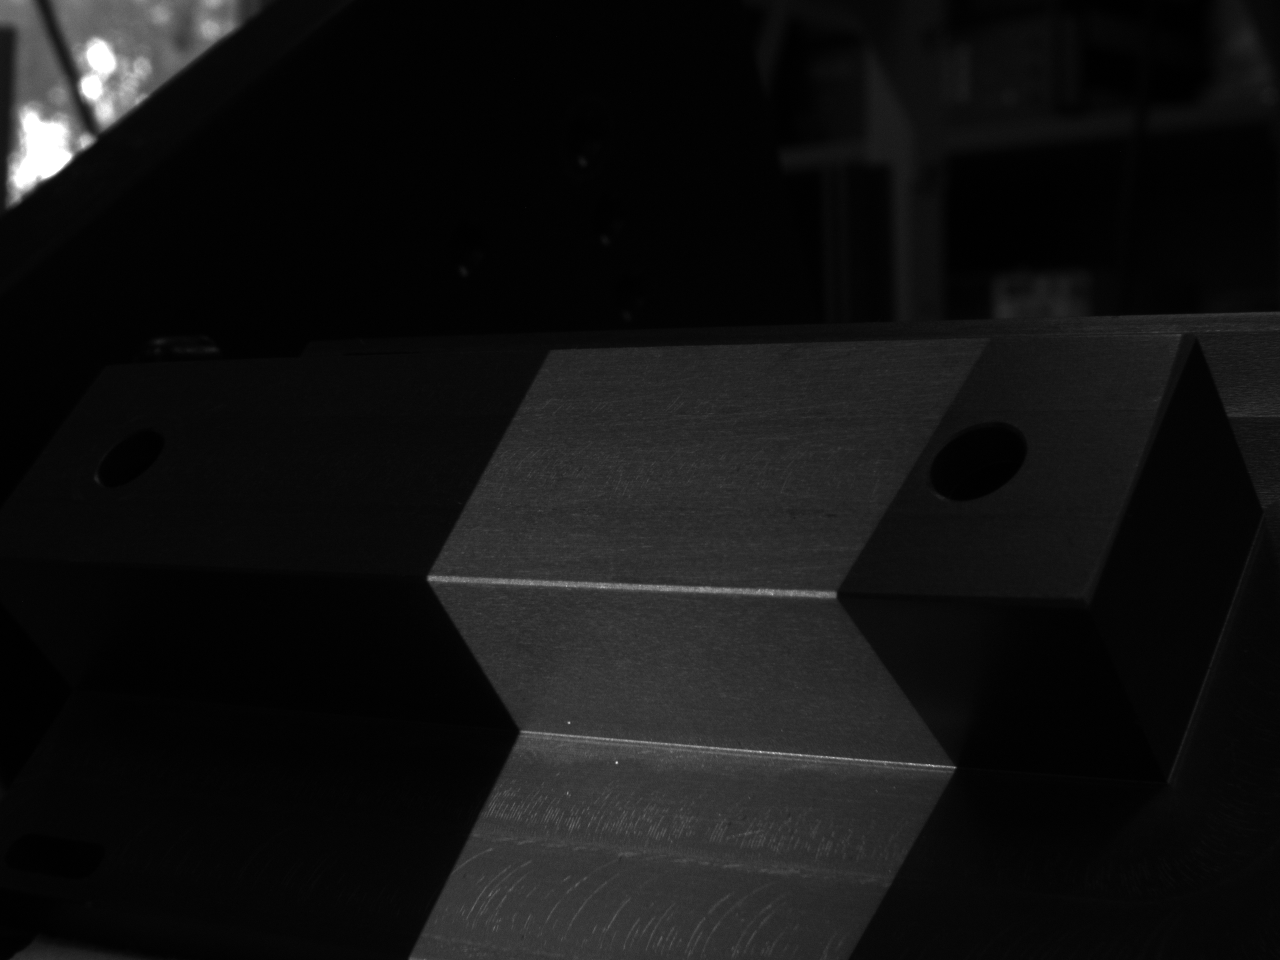
\includegraphics[width=0.49\linewidth]{images/snapshots_scan/SIMULATED-RIGHT-PGR-SN9041369/gray_09_inv}
        }
        \caption{Cámara derecha: 5 últimos patrones proyectados (izq.) y su inverso (der.)}
        \label{fig:ejemploProyeccionCamaraDerecha5a9}
\end{figure}

En la imagen superior de la \autoref{fig:ejemploDecodificacion} se puede observar el resultado de la decodificación para las imágenes del ejemplo. En la imagen inferior se muestra el resultado de un primer procesamiento de la imagen decodificada. Al usar patrones binarios, la única información útil es la representada por el límite entre una franja y la siguiente. Es decir, el valor del código de cualquier pixel dentro de una franja de pixels con el mismo código no nos brinda información relevante (nos sirve para establecer que ese pixel corresponde a una parte de la pieza, pero no contiene información relevante para conocer con exactitud su ubicación en el espacio). Es por esto que lo primero que se realiza es obtener la ubicación de los \emph{bordes} entre las franjas. Los únicos bordes que son realmente útiles son aquellos que se encuentran entre dos franjas con código sucesivo. 

A partir de este procesamiento se generan listas de pixeles correspondientes a los límites entre franjas sucesivas. Como ejemplo se genera una lista de los pixels correspondientes al límite entre las franjas con código 1 y 2, otra lista para los pixels correspondientes al límite entre las franjas con código 2 y 3, y así sucesivamente. Esto se realiza para las imagenes decodificadas de cada cámara utilizada.
Para observar la analogía con un escaner de línea, se puede decir que cada lista de pixels es el equivalente a una línea decodificada en un escáner de línea. De esta manera una de las ventajas de los métodos de luz estructuradas es evidente: con el uso de patrones binarios de 10 bits (en nuestro caso, $10 x 2 + 2 = 22$ imagenes) se puede obtener el equivalente a $2^{10} - 1 = 1023$ (descartando los límites exteriores de las franjas de los extremos) o $2^{10} + 1 = 1025$ (utilizando los límites exteriores de las franjas de los extremos) perfiles de un escaner de línea (donde se necesita una imagen para cada perfil).

\begin{figure}[!bth]
    \myfloatalign
        \subfloat[Decodificación]{
            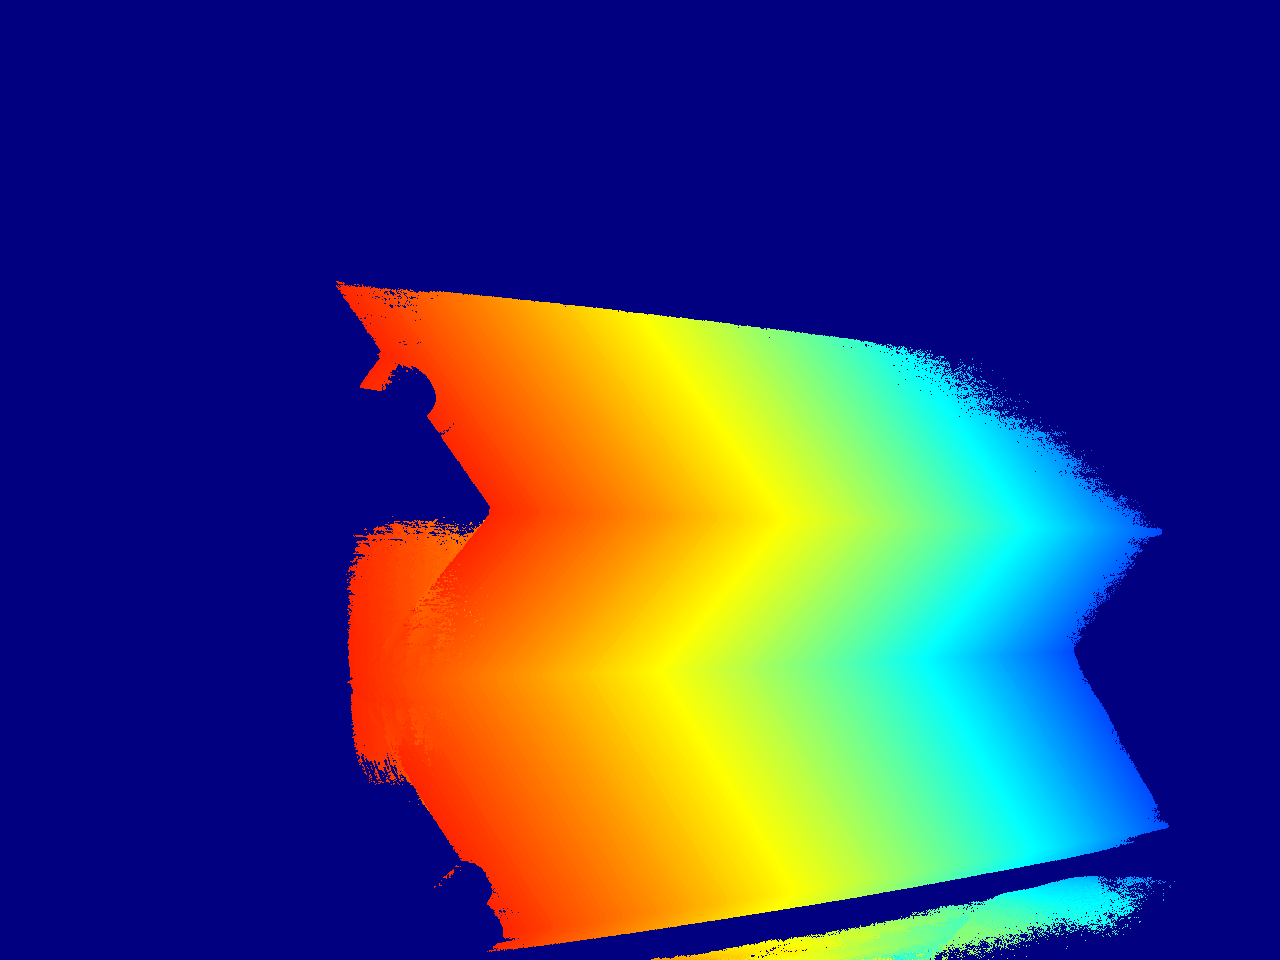
\includegraphics[width=0.49\linewidth]{images/soft/decodedLeft}
            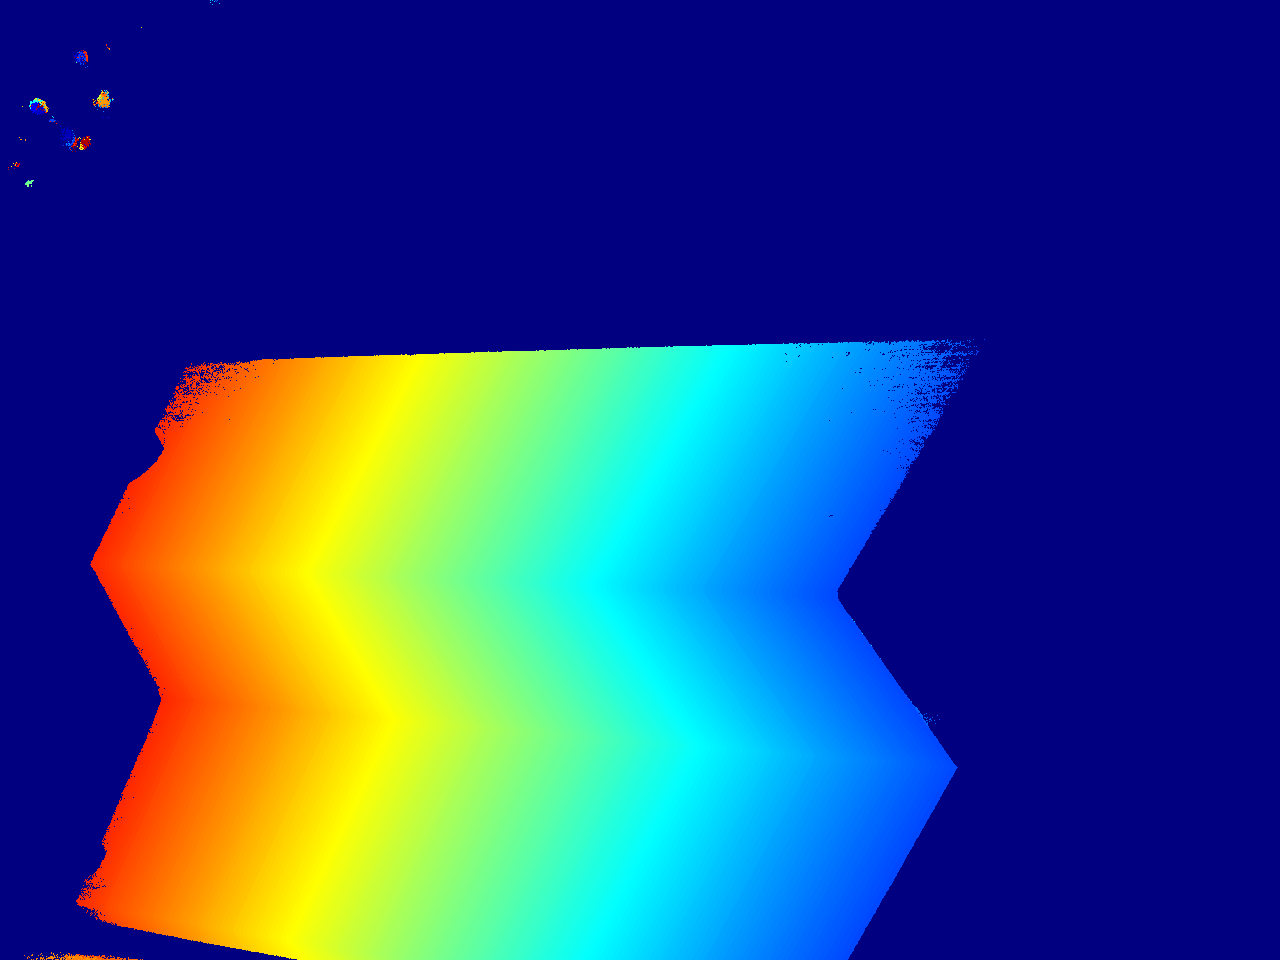
\includegraphics[width=0.49\linewidth]{images/soft/decodedRight}
        }
        \\
        \subfloat[Sólo bordes]{
            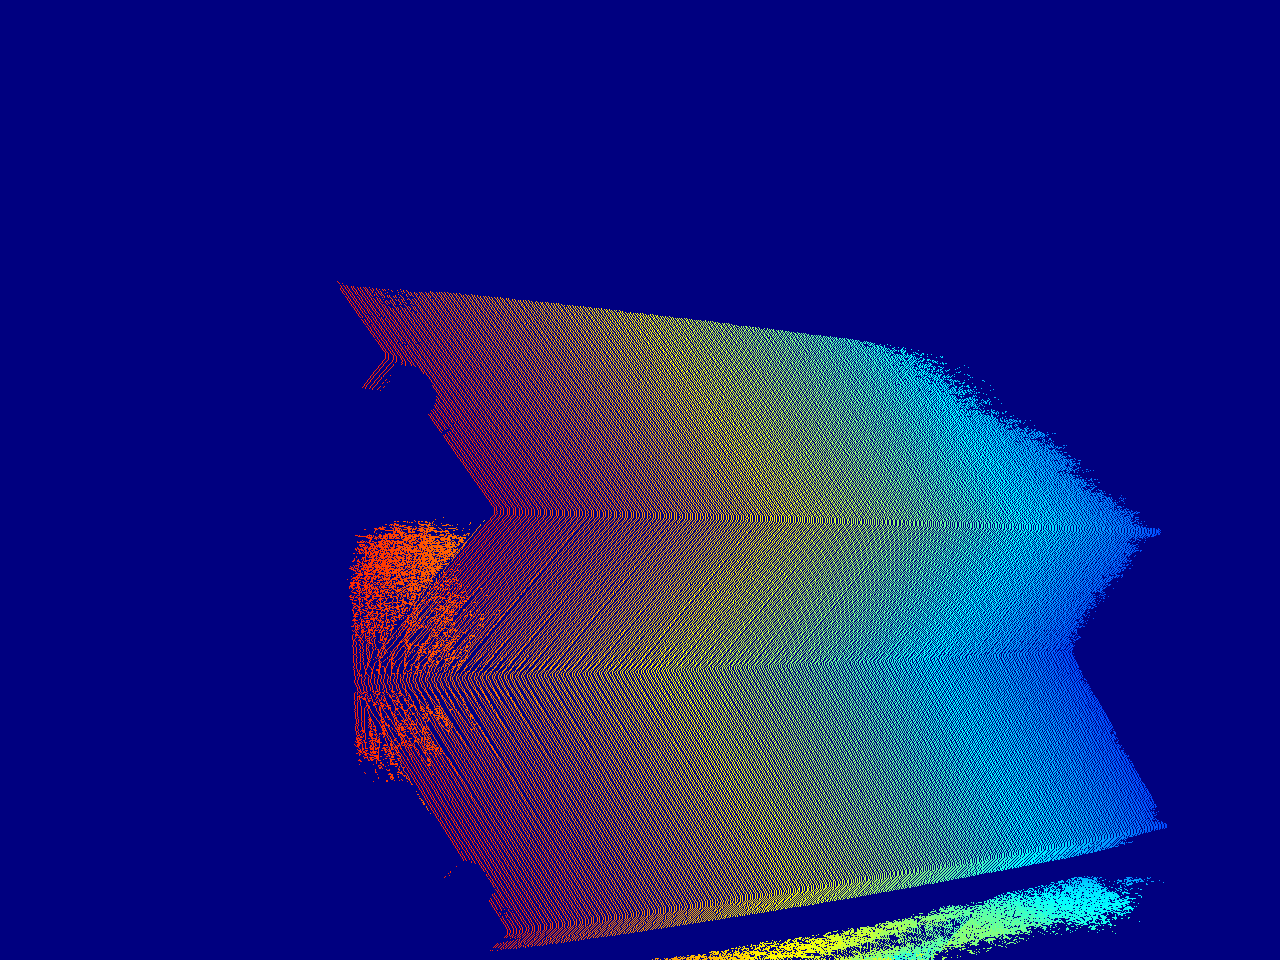
\includegraphics[width=0.49\linewidth]{images/soft/decodedBordersLeft}
            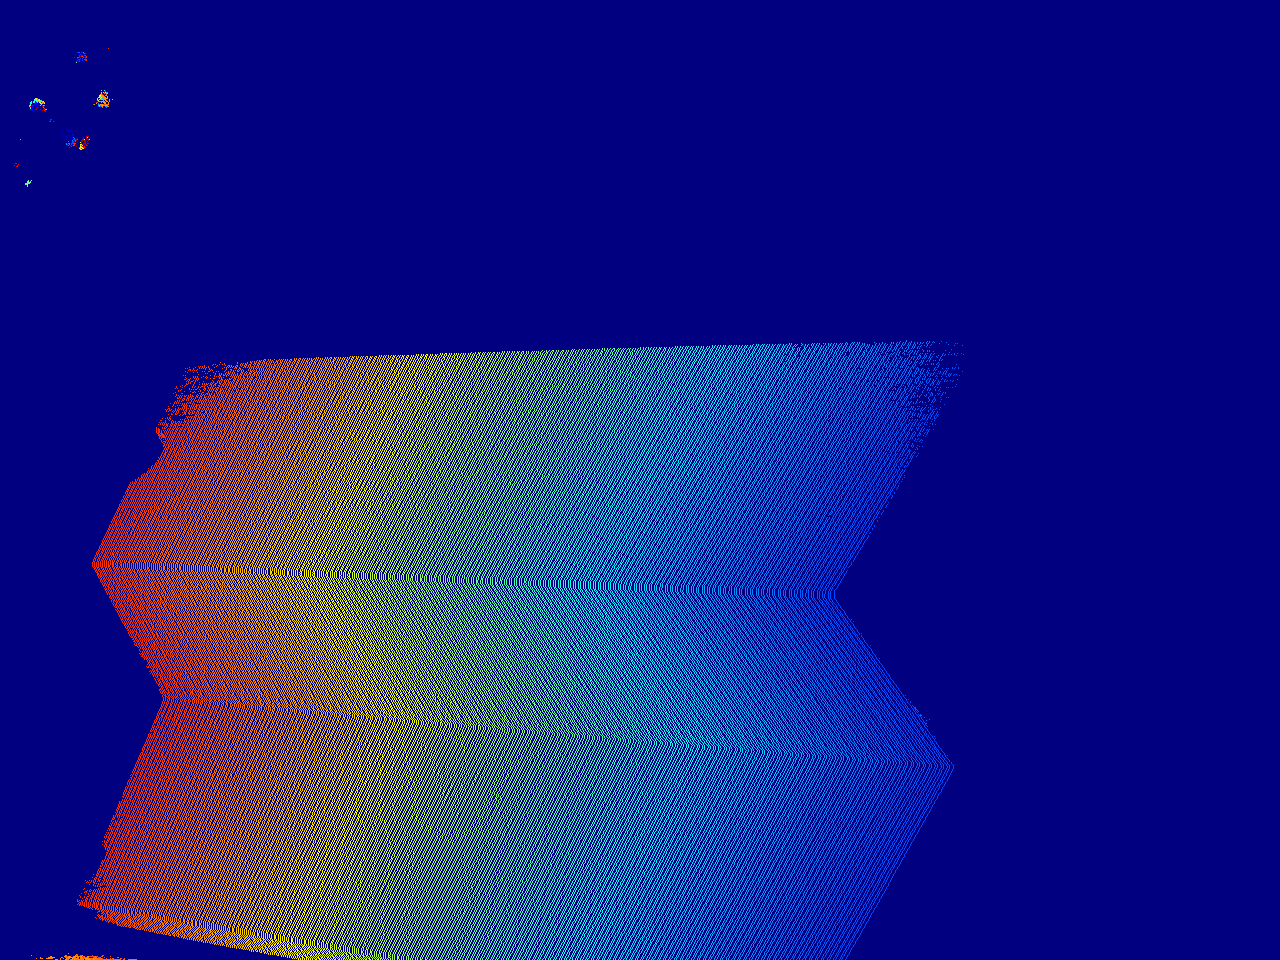
\includegraphics[width=0.49\linewidth]{images/soft/decodedBordersRight}
        }
        \caption{Resultado de la decodificación de los patrones}
        \label{fig:ejemploDecodificacion}
\end{figure}



\section{Reconstrucción}
- matcheo de las franjas detectadas por cada cámara

- aprovechar geometría epipolar

- obtención de la nube de puntos 3D

\begin{figure}[!bth]
    \myfloatalign
        \subfloat{
            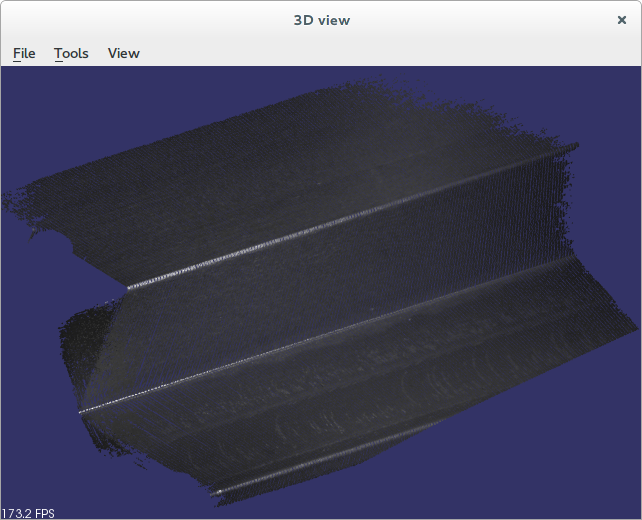
\includegraphics[width=0.8\linewidth]{images/soft/screenshot3DView}
        }
        \\
        \subfloat{
            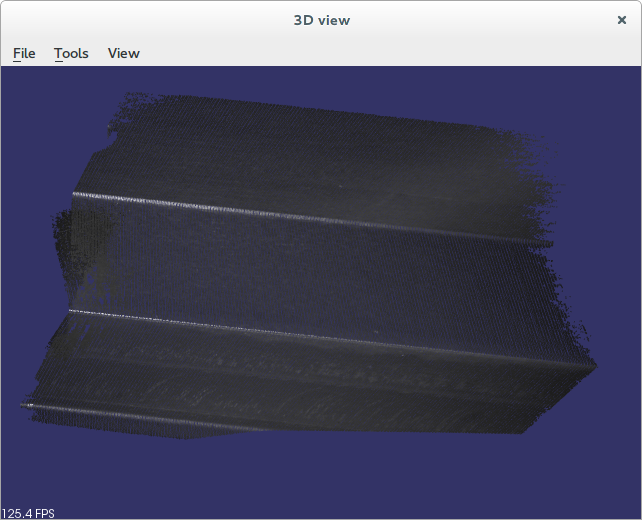
\includegraphics[width=0.8\linewidth]{images/soft/screenshot3DView2}
        }
        \\
        \subfloat{
            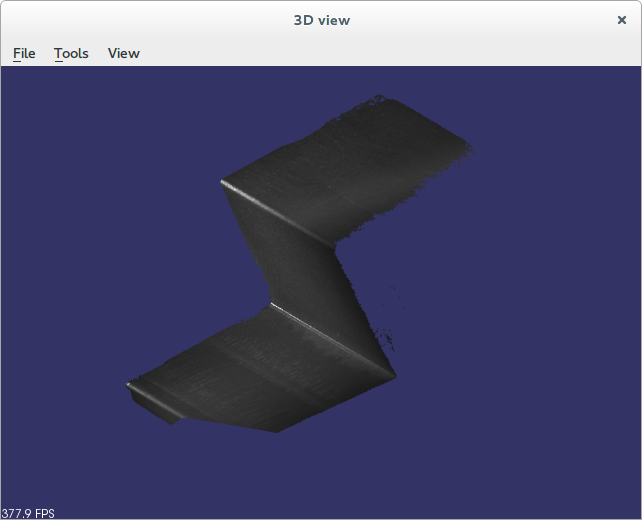
\includegraphics[width=0.8\linewidth]{images/soft/screenshot3DView3}
        }
        \caption{Visualización de la nube de puntos 3D}
        \label{fig:ejemploVisualizacionNubePuntos}
\end{figure}

\section{Calibración del dispositivo}
- método y programa de calibración

\section{Limitaciones}

- problema de superficie brillosa

%*****************************************
%*****************************************
%*****************************************
%*****************************************
%*****************************************




